%% March 2018
%%%%%%%%%%%%%%%%%%%%%%%%%%%%%%%%%%%%%%%%%%%%%%%%%%%%%%%%%%%%%%%%%%%%%%%%%%%%
% AGUJournalTemplate.tex: this template file is for articles formatted with LaTeX
%
% This file includes commands and instructions
% given in the order necessary to produce a final output that will
% satisfy AGU requirements, including customized APA reference formatting.
%
% You may copy this file and give it your
% article name, and enter your text.
%
%%%%%%%%%%%%%%%%%%%%%%%%%%%%%%%%%%%%%%%%%%%%%%%%%%%%%%%%%%%%%%%%%%%%%%%%%%%%
% PLEASE DO NOT USE YOUR OWN MACROS
% DO NOT USE \newcommand, \renewcommand, or \def, etc.
%
% FOR FIGURES, DO NOT USE \psfrag or \subfigure.
% DO NOT USE \psfrag or \subfigure commands.
%%%%%%%%%%%%%%%%%%%%%%%%%%%%%%%%%%%%%%%%%%%%%%%%%%%%%%%%%%%%%%%%%%%%%%%%%%%%
%
% Step 1: Set the \documentclass
%
% There are two options for article format:
%
% PLEASE USE THE DRAFT OPTION TO SUBMIT YOUR PAPERS.
% The draft option produces double spaced output.
%

%% To submit your paper:
%\documentclass[draft,linenumbers]{agujournal2018}
\documentclass[draft]{agujournal2018} % pri removed linenumbers
\usepackage{apacite}
\usepackage{url} %this package should fix any errors with URLs in refs.
\usepackage{longtable,booktabs}
\usepackage{float}

%%%%%%%
%\usepackage{trackchanges}
% uncomment the line above to use the TrackChanges package to mark revisions if needed.
% The trackchanges package adds five new LaTeX commands:
%
%  \note[editor]{The note}
%  \annote[editor]{Text to annotate}{The note}
%  \add[editor]{Text to add}
%  \remove[editor]{Text to remove}
%  \change[editor]{Text to remove}{Text to add}
%
% complete documentation is here: http://trackchanges.sourceforge.net/
%%%%%%%

\draftfalse
%\pagestyle{empty} % pri to remove the header
% Now, type in the journal name: \journalname{<Journal Name>}

% ie, \journalname{Journal of Geophysical Research}
%% Choose from this list of Journals:
%
% JGR-Atmospheres
% JGR-Biogeosciences
% JGR-Earth Surface
% JGR-Oceans
% JGR-Planets
% JGR-Solid Earth
% JGR-Space Physics
% Global Biochemical Cycles
% Geophysical Research Letters
% Paleoceanography
% Radio Science
% Reviews of Geophysics
% Tectonics
% Space Weather
% Water Resource Research
% Geochemistry, Geophysics, Geosystems
% Journal of Advances in Modeling Earth Systems (JAMES)
% Earth's Future
% Earth and Space Science
% Geohealth
%

\journalname{Water Resources Research}

\begin{document}

%% ------------------------------------------------------------------------ %%
%  Title
%
% (A title should be specific, informative, and brief. Use
% abbreviations only if they are defined in the abstract. Titles that
% start with general keywords then specific terms are optimized in
% searches)
%
%% ------------------------------------------------------------------------ %%

% Example: \title{This is a test title}

\title{A feature-based procedure for detecting technical outliers in water-quality data from in situ sensors}

%% ------------------------------------------------------------------------ %%
%
%  AUTHORS AND AFFILIATIONS
%
%% ------------------------------------------------------------------------ %%

% Authors are individuals who have significantly contributed to the
% research and preparation of the article. Group authors are allowed, if
% each author in the group is separately identified in an appendix.)

% List authors by first name or initial followed by last name and
% separated by commas. Use \affil{} to number affiliations, and
% \thanks{} for author notes.
% Additional author notes should be indicated with \thanks{} (for
% example, for current addresses).

% Example: \authors{A. B. Author\affil{1}\thanks{Current address, Antartica}, B. C. Author\affil{2,3}, and D. E.
% Author\affil{3,4}\thanks{Also funded by Monsanto.}}

\authors{Priyanga Dilini Talagala\affil{1,2}, Rob J. Hyndman\affil{1,2}, Catherine Leigh\affil{1,3}, Kerrie Mengersen\affil{1,4}, Kate Smith-Miles\affil{1,5}}

\affiliation{1}{ARC Centre of Excellence for Mathematics and
Statistical Frontiers (ACEMS), Australia}
\affiliation{2}{Department of Econometrics and Business Statistics, Monash University,
Australia}
\affiliation{3}{Institute for Future Environments, Science and Engineering Faculty, Queensland University of Technology, Australia}
\affiliation{4}{School of Mathematical Sciences, Science and Engineering Faculty, Queensland University of Technology, Australia}
\affiliation{5}{School of Mathematics and Statistics, University of Melbourne, Australia}

%\affiliation{=number=}{=Affiliation Address=}
%(repeat as many times as is necessary)

%% Corresponding Author:
% Corresponding author mailing address and e-mail address:

% (include name and email addresses of the corresponding author. More
% than one corresponding author is allowed in this LaTeX file and for
% publication; but only one corresponding author is allowed in our
% editorial system.)

% Example: \correspondingauthor{First and Last Name}{email@address.edu}

\correspondingauthor{Priyanga Dilini Talagala}{dilini.talagala@monash.edu}

%% Keypoints, final entry on title page.

% Example:
% \begin{keypoints}
% \item	List up to three key points (at least one is required)
% \item	Key Points summarize the main points and conclusions of the article
% \item	Each must be 100 characters or less with no special characters or punctuation
% \end{keypoints}

%  List up to three key points (at least one is required)
%  Key Points summarize the main points and conclusions of the article
%  Each must be 100 characters or less with no special characters or punctuation

\begin{keypoints}
\item  Our feature-based procedure  starts by applying different statistical transformations to water-quality data to highlight outliers in high dimensional space
\item  Density and distance-based unsupervised outlier scoring techniques were  applied to detect outliers due to technical issues with the sensors
\item  An approach based on extreme value theory was then used to calculate outlier thresholds
\end{keypoints}



%% ------------------------------------------------------------------------ %%
%
%  ABSTRACT
%
% A good abstract will begin with a short description of the problem
% being addressed, briefly describe the new data or analyses, then
% briefly states the main conclusion(s) and how they are supported and
% uncertainties.
%% ------------------------------------------------------------------------ %%

%% \begin{abstract} starts the second page
\newpage
\begin{abstract}
Outliers due to technical errors in water quality data from
\emph{in~situ} sensors can reduce data quality and have a direct impact
on inference drawn from subsequent data analysis. However, outlier
detection through manual monitoring is infeasible given the volume and
velocity of data the sensors produce. Here, we introduce an automated  procedure, named oddwater  that provides early detection of outliers in water-quality
data from \emph{in~situ} sensors caused by technical issues. Our oddwater procedure  is used to first identify the data features that
differentiate outlying instances from typical behaviours. Then
statistical transformations are applied to make the outlying instances
stand out in a transformed data space. Unsupervised outlier scoring
techniques are applied to the transformed data space and an
approach based on extreme value theory is used to calculate a threshold
for each potential outlier. Using two datasets obtained from
\emph{in~situ} sensors in rivers flowing into the Great Barrier Reef
lagoon, Australia, we show that \color{black} oddwater \color{black} successfully identifies outliers involving abrupt changes in turbidity, conductivity and river level, including sudden spikes, sudden isolated drops and level shifts, while maintaining very low false detection rates. We have implemented this \color{black} oddwater procedure \color{black} in the open source R package \texttt{oddwater}.
\end{abstract}

%% ------------------------------------------------------------------------ %%
%
%  TEXT
%
%% ------------------------------------------------------------------------ %%

%%% Suggested section heads:
% \section{Introduction}
%
% The main text should start with an introduction. Except for short
% manuscripts (such as comments and replies), the text should be divided
% into sections, each with its own heading.

% Headings should be sentence fragments and do not begin with a
% lowercase letter or number. Examples of good headings are:

% \section{Materials and Methods}
% Here is text on Materials and Methods.
%
% \subsection{A descriptive heading about methods}
% More about Methods.
%
% \section{Data} (Or section title might be a descriptive heading about data)
%
% \section{Results} (Or section title might be a descriptive heading about the
% results)
%
% \section{Conclusions}

\section{Introduction}\label{introduction}

Water-quality monitoring traditionally relies on water samples collected
manually. The samples are then analyzed within laboratories to determine
the water-quality variables of interest. This type of rigorous
laboratory analysis of field-collected samples is crucial in making
natural resources management decisions that affect human welfare and
environmental conditions. However, with the rapid advances in hardware
technology, the use of \emph{in~situ} water-quality sensors positioned
at different geographic sites is becoming an increasingly common
practice used to acquire real-time measurements of environmental and
water-quality variables. Though only a subset of the required
water-quality variables can be measured by these sensors, they have
several advantages. Their ability to collect large quantities of data
and to archive historic records allows for deeper analysis of
water-quality variables to improve understanding about field
conditions and water-quality processes \citep{glasgow2004real}.
Near-real-time monitoring also allows operators to identify and
respond to potential issues quickly and thus manage the operations
efficiently. Further, the use of \emph{in~situ} sensors can greatly
reduce the labor involved in field sampling and laboratory analysis.

Water-quality sensors are exposed to changing environments and extreme
weather conditions, and thus are prone to errors, including failure.
Automated detection of outliers in water-quality data from
\emph{in~situ} sensors has therefore captured the attention of many
researchers both in the ecology and data science communities
\citep{hill2009real,archer2003fault, raciti2012anomaly, mckenna2007event, koch2010distributed}. This problem of outlier detection in water-quality
data from \emph{in~situ} sensors can be divided into two sub-topics
according to their focus: (1) identifying errors in the
data due to issues unrelated to water events per se, such as technical
aberrations, that make the data unreliable and untrustworthy; and (2)
identifying real events (e.g.~rare but sudden spikes in turbidity
associated with rare but sudden high-flow events). Both problems are
equally important when making natural resource management decisions that
affect human welfare and environmental conditions. Problem 1 can also be
considered as a data preprocessing phase before addressing Problem 2.

In this work we focus on Problem 1, i.e. detecting unusual
measurements caused by technical errors that make data unreliable
and untrustworthy, and affect performance of any subsequent data
analysis under Problem 2. According to \citet{yu2012bayesian}, the
degree of confidence in the sensor data is one of the main requirements
for a properly defined environmental analysis procedure. For instance,
researchers and policy makers are unable to use water-quality data
containing technical outliers with confidence for decision making and
reporting purposes, because erroneous conclusions regarding the quality
of the water being monitored could ensue, leading, for example, to
inappropriate or unnecessary water treatment, land management or warning
alerts to the public
\citep{kotamaki2009wireless,rangeti2015validity}. Missing values and
corrupted data can also have an adverse impact on water-quality model
building and calibration processes \citep{archer2003fault}. Early
detection of these technical outliers will limit the use of corrupted
data for subsequent analysis. For instance, it will limit the use of
corrupted data in real-time forecasting and online applications such as
on-line drinking water-quality monitoring and early warning systems
\citep{storey2011advances}, predicting algal bloom outbreaks leading
to fish kill events and potential human health impacts, forecasting
water level and currents etc.
\citep{glasgow2004real,archer2003fault,hill2006automated}. However,
because data arrive near continuously at high speed in large quantities,
manual monitoring is highly unlikely to be able to capture all the
errors. These issues have therefore increased the importance of
developing automated methods for early detection of outliers in
water-quality data from \emph{in~situ} sensors \citep{hill2009real}.

Different statistical approaches are available to detect outliers in
water-quality data from \emph{in situ} sensors. For example,
\citet{hill2006automated} addressed the problem of outlier detection
in environmental sensors using regression-based time series models. In
this work they addressed the scenario as a univariate problem. Their
prediction models are based on four data-driven methods: naive,
clustering, perceptron, and Artificial Neural Networks (ANN).
Measurements that fell outside the bounds of an established prediction
interval were declared as outliers. They also considered two strategies:
anomaly detection (AD) and anomaly detection and mitigation (ADAM) for
the detection process. ADAM replaces detected outliers with the
predicted value prior to the next predictions whereas AD simply uses the
previous measurements without making any alteration to the detected
outliers. These types of data-driven methods develop models using sets
of training examples containing a feature set and a target output.
Later, \citet{hill2009real} addressed the problem by developing three
automated anomaly detection methods using dynamic Bayesian networks
(DBN) and showed that DBN-based detectors using either robust Kalman
filtering or Rao-Blackwellized particle filtering, outperformed that of
Kalman filtering.

Another common approach for detecting outliers in environmental sensor
data is based on residuals (the differences between predicted and actual
values). Due to the ability of ANNs to model a wide range of complex
non-linear phenomena, \citet{moatar1999ph} used ANN techniques to
detect anomalies such as abnormal values, discontinuities, and drifts in
pH readings. After developing the pH model, the Student t-test and the
cumulative Page--Hinkley test were applied to detect changes in the mean
of the residuals to detect measurement error occurring over short
periods of time. The work was later expanded to a
multivariate scenario with some additional water-quality variables
including dissolved oxygen, electrical conductivity, pH and temperature  \citep{moatar2001quality}. Their proposed algorithm used both deterministic and stochastic approaches for the model building process. Observed data were then compared with the model forecasts using a set of classical statistical
tests to detect outliers, demonstrating the
effectiveness and advantages of the multimodel approach. Later,
\citet{archer2003fault} proposed a method to detect failures in the
water-quality sensors due to biofouling based on a sequential likelihood
ratio test. Their method also had the ability to provide estimates of
biofouling onset time, which was useful for the subsequent step of
outlier correction.

A common feature of all of the above methods is that they are usually
employed in a supervised or semi-supervised context and thus require training data pre-labeled with known outliers  or data that are free from the anomalous features
of interest. In many cases, however, not all the possible outliers are
known in advance and can arise spontaneously as new outlying behaviors
during the test phase. In such situations, supervised methods may fail
to detect those outliers. Semi-supervised methods are also unsuitable
for certain applications due to the unavailability of training data
containing only typical instances that are free from outliers
\citep{goldstein2016comparative}. The datasets that we consider in
this paper suffer from both of these limitations highlighting
the need for a more general approach.

\color{black}

This paper develops a method for detecting technical outliers in water-quality data derived from  \emph{in~situ} sensors. Prior work by \citet{leigh2019framework} emphasises the importance of different anomaly types and end-user needs and provides the starting point for constructing a framework for automated anomaly detection in high frequency water-quality data from \emph{in~situ} sensors. Their work briefly introduced unsupervised feature based methods for detecting technical-outliers in such data. The present paper differs substantially from \citet{leigh2019framework} as (1) the unsupervised feature based procedure we present for detecting technical-outliers in high frequency water-quality data measured by \emph{in situ} sensors is its sole focus  (2) the unsupervised feature based procedure is fully elaborated in both details and depth and (3) the experimental results are enhanced through emphasis on the multivariate capabilities of the unsupervised feature based procedure. Furthermore, we focus on outliers involving abrupt changes in value, including sudden spikes, sudden isolated drops and level shifts (high priority outliers as described in \citet{leigh2019framework}) rather than the broader suite considered by \citet{leigh2019framework}.

First, we present in detail our unsupervised feature based procedure that provides early detection of technical outliers in water-quality data from \emph{in~situ} sensors. \color{black}  Rule-based methods are also incorporated into the procedure to flag occurrences of impossible, out-of-range, and missing values. Second, we provide a comparative analysis of the efficacy and reliability of both density- and nearest neighbor distance-based outlier scoring techniques. Third, we introduce an R \citep{Rsoftware} package, \texttt{oddwater} \citep{oddwater2018} that implements the  feature-based procedure and related functions. \color{black} Further, to facilitate reproducibility and reuse of the results presented in this paper we have  made all of the code and associated  datasets available on zenodo\footnote{DOI: 10.5281/zenodo.2890469}.

 \color{black}Our feature-based procedure  \color{black} has many advantages: (1) it can take the correlation structure of the water-quality variables into account when
detecting outliers; (2) it can be applied to both univariate and
multivariate problems; (3) the outlier scoring techniques that we
consider are unsupervised, data-driven approaches and therefore do not
require training datasets for the model building process, and can be
extended easily to other time series from other sites; (4) the outlier
thresholds have a probabilistic interpretation as they are based on
extreme value theory; (5) the  \color{black} approach \color{black}  has the ability to deal with irregular (unevenly spaced) time series; and (6) \color{black} it can easily be extended to streaming data. In contrast to a batch scenario, which assumes that the entire dataset is available prior to the analysis with the focus on detecting complete events, the streaming data scenario gives many additional challenges due to high velocity, unbounded, nonstationary data with incomplete events \citep{hill2009real, talagala2018anomaly}. In this paper, although our oddwater procedure is introduced as a batch method it \color{black} can easily be extended to streaming data such that it can provide near-real-time support \color{black} using a sliding window technique. \color{black}

\section{Materials and Methods}\label{sec:methodology}

Our \color{black} unsupervised feature-based procedure \color{black} for detecting outliers in water-quality data from
\emph{in situ} sensors has six main steps (Figure
\ref{fig:frameworkwater}), and the structure of this section is organised
accordingly. \color{black} For easy reference, we named our unsupervised feature-based procedure as oddwater procedure, which stands for “\textbf{O}utlier \textbf{D}etection in \textbf{D}ata from \textbf{WATER}-quality sensors” \color{black}

\begin{figure}[H]

{\centering 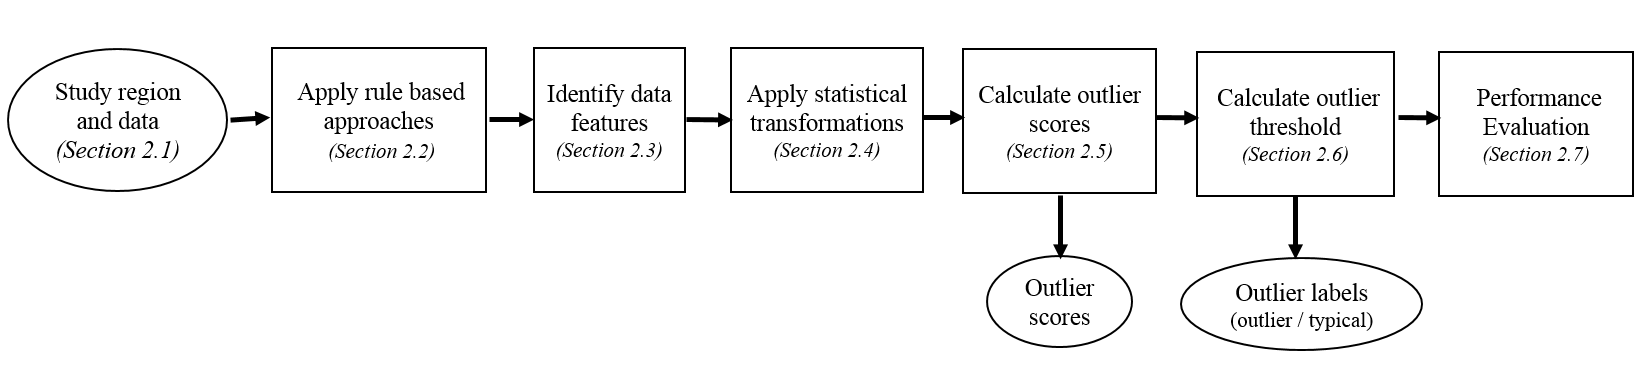
\includegraphics[width=1\linewidth]{./fig/framework}
}
\caption{\color{black} Unsupervised feature-based procedure, named oddwater procedure \color{black} for outlier detection in water quality data from \textit{in situ} sensors. Squares represents the main steps involved. Circles correspond to input and output. }\label{fig:frameworkwater}
\end{figure}

\subsection{Study region and data}\label{study-region-and-data}

To evaluate the effectiveness of our \color{black} oddwater procedure \color{black} we considered a
challenging real-world problem of monitoring water-quality using \emph{in situ} sensors in a natural river system. This is
challenging because the system is susceptible to a wide range of
environmental, biological and human impacts that can lead to variation
in water-quality and affect the technological performance of the
sensors. For comparison, we evaluated two study sites, Sandy Creek and
Pioneer River (PR), both in the Mackay-Whitsunday region of northeastern
Australia \citep{mitchell2005sediments}. These two rivers flow into
the Great Barrier Reef lagoon, and have catchment areas of 1466 km\(^2\)
and 326 km\(^2\), respectively. In this region, the wet season typically
occurs from December to April and is dominated by higher rainfall and
air temperatures, whereas the dry season typically occurs from May to
November with lower rainfall and air temperatures
\citep{mcinnes2015wet}. The sensors at these two sites are housed
within a monitoring station on the river banks. Water is pumped from the rivers to the stations approximately every 60 or 90 minutes to
take measurements of various water-quality variables that are logged by
the sensors. Here we focused on three water-quality variables: turbidity(NTU), \color{black} conductivity (strictly, specific conductance at \(25^0\)C; \(\mu\)S/cm) \color{black} and river level (m).

The water-quality data obtained from \emph{in~situ} sensors located at
Sandy Creek were available from 12 March 2017 to 12 March 2018. The data
set included 5402 recorded points. These time series were irregular
(i.e.~the frequency of observations was not constant) with a minimum
time gap of 10 minutes and a maximum time gap of around 4 hours. The data
obtained from Pioneer River were available from 12 March 2017 to 12
March 2018, and included 6280 recorded points. Many missing values were
observed during the initial part of all three series, turbidity, conductivity and river level, at Pioneer River. \color{black}  With the help of a group of water-quality experts, familiar with the study region and with over 40 years of combined knowledge of river water quality, observations were labeled as outliers or not, with the aim of evaluating the performance of the procedure. Our Shiny web application available through the \emph{oddwater} R package was  used during the labeling process to pinpoint observations and provide greater visual insight into the data. Using this interactive visualization tool and expert knowledge, the ground-truth labels were decided by consensus vote. \color{black}

\subsection{Apply rule-based
approaches}\label{apply-rule-based-approaches}

 \color{black} Following \citet{thottan2003anomaly}, we incorporated simple rules
into our oddwater procedure to detect outliers such as
out-of-range values, impossible values (e.g.~negative values) and
missing values, and labeled them prior to applying the
statistical transformations introduced in Section \ref{sec:trans}. \color{black}

If a sensor reading was outside the corresponding sensor detection range
it was marked as an outlier. Negative readings are also inaccurate and
impossible for river turbidity, conductivity and level. We therefore
imposed a simple constraint on the algorithm to filter these values and
mark them as outliers. Missing values are also frequently encountered in
water-quality sensor data \citep{rangeti2015validity}. We detected
missing values by calculating the time gaps between readings. If a gap
exceeded the maximum allowable time difference between any two
consecutive readings, the corresponding time stamp was then marked as an
outlier due to missingness. \color{black} Here, the maximum allowable time difference was set at 180 minutes, given that the water-quality measurements were set to be taken at most every 90 minutes (measurements were often taken at higher frequencies during high-flow events, e.g. every 10-15 minutes, and occasionally as one-off measurements at times of interest to water managers). \color{black}

\subsection{Identify data features}\label{identify-data-features}

\color{black} After labeling out-of-range, impossible and missing values as outliers, further investigation was done with the remaining observations. We initiated this investigation by identifying  common characteristics or patterns of the possible types of outliers in water-quality data that would differentiate them from typical instances or events. \color{black} For turbidity, for example, ``extreme" deviations upward are more likely than deviations downwards
\citep{panguluri2009distribution}. The opposite is true for
conductivity \citep{tutmez2006modelling}. Further, in a turbidity
time series a sudden isolated upward shift (spike) is a point outlier (a
single observation that is surprisingly large, independent of
the neighboring observations \citep{goldstein2016comparative}), but
if the sudden upward shift is followed by a gradually decaying tail then
it becomes part of the typical behavior. For river level, rates of rise
are often fast compared with fall rates. In general, isolated data
points that are outside the general trend are outliers. Further, natural
water processes under typical conditions generally tend to be
comparatively slow; sudden changes therefore mostly correspond to
outlying behaviors. Hereafter, these characteristics will be referred to as
`data features'.

\subsection{Apply statistical transformations}\label{sec:trans}

After identifying the data features, different statistical
transformations were applied to the time series to highlight different
types of outliers, focusing on sudden isolated spikes, sudden isolated
drops, sudden shifts, and clusters of spikes (Table \ref{table:table_1})
that deviate from the typical characteristics of each variable
\citep{leigh2019framework}.

\begin{table}[!htbp]
\footnotesize
\caption{Transformation methods used to highlight different types of outliers in water-quality sensor data. Let $Y_t$ represent an original series from one of the three variables: turbidity, conductivity and level at time $t$.}
\label{table:table_1}
\tabcolsep=0.12cm
\begin{tabular}{p{3cm}p{3cm}p{4cm}p{4cm}}
\toprule
\textbf{Transformation}
  & \textbf{Formula}
  & \textbf{Data Feature}
  & \textbf{Focus} \\
\midrule
Log transformation
  & $\log(y_{t})$
  & High variability of the data.
  & To stabilize the variance across time series and make the patterns more visible (e.g.\ level shifts)
\\\midrule
First difference
  & $\log(y_{t} /y_{t-1})$
  & Isolated spikes (in both positive and negative directions) that are outside the general trend are considered as outliers. Under typical behavior, sudden upward (downward) shifts are possible for turbidity (conductivity), but their rate of fall (rise) is generally slower than the rate of rise (fall).
  & To separate isolated spikes from the general upward/downward trend patterns.
\\\midrule
Time gap
  & $\Delta t$
  &
  & To identify missing values.
\\\midrule
First derivative
  & $x_t = \log(y_{t} /y_{t-1}) / \Delta t$
  & Data are unevenly spaced time series.
  & To handle irregular time series. Data points with large gaps will get small value. Large gaps indicate the lack of information to make a claim regarding the points.
\\\midrule
One sided derivative
\\
\quad   \textit{Turbidity or level}
  & $\min\{x_t, 0\}$
  & Extreme upward trend in turbidity and level under typical behavior.
  & To separate spikes from typical upward trends. \\
\quad   \textit{Conductivity}
  & $\max\{x_t, 0\}$
  & Extreme downward trend in conductivity under typical behavior.
  & To separate isolated drops from typical downward trends.
\\\midrule
Rate of change
  & $(y_{t} - y_{t-1}) / y_{t}$
  & High or low variability in the data.
  & To detect change points in variance.
  \\\midrule
Relative difference
  & $y_{t} - (1/2)(y_{t-1} + y_{t+1})$
  &Natural processes are comparatively slow. Sudden changes (upward or downward movements) typically correspond to outlying instances.
  & To detect sudden changes (both upward and downward movements)
\\\bottomrule
\end{tabular}
\end{table}

In this work we considered the outlier detection problem in a
multivariate setting. By applying different transformations on
water-quality variables we converted our original problem of outlier
detection in the temporal context to a non-temporal context through a
high dimensional data space \color{black} with three dimensions defined by the three variables: turbidity, conductivity and river level.
Different transformations were applied on different axes of the three dimensional data space resulting in different data patterns. We evaluated the performance
of the transformations \citep{dang2014transforming} using the
maximum separability of the two classes: outliers and typical points in the three dimensional data space. For example, in the data obtained from Sandy Creek, the one sided derivative transformation clearly separated all of the target outlying points from the typical points, shown as either red triangles (corresponding to outliers) or green squares (corresponding to the immediate neighbours of outliers)  (Figure~\ref{fig:transformTypePng}(e)). To provide a better visual illustration, in Figure~\ref{fig:transformTypePng}, we present only the two dimensional data space defined by turbidity and conductivity; however our actual data space is three dimensional. In this work our focus was to evaluate whether each point in time is an outlier or not, such that an alarm could be triggered in the presence of an outlier. However, it was not our interest to investigate which variable(s) is (are) responsible for the outlier in time. Therefore, in Figure~\ref{fig:transformTypePng}, a point is marked as an outlier in the two dimensional space if at least one variable corresponding to that point was labelled as an outlier by the water-quality experts. \color{black}

\color{black} When the transformation involves both the current value \(Y_{t}\) and
the lagged value \(Y_{t-1}\) (as in the first difference, first
derivative, and one sided derivatives), the neighboring points can
emerge as outliers instead of the actual outlying point. For an example,
if an outlier occurs at time point \(t\), then the two values derived
from the first derivative transformation (\((y_{t} - y_{t-1})\) and
\((y_{t+1}-y_{t})\)) get highlighted as outlying values because they both
involve \(y_{t}\). \color{black} That is each outlying instance is now represented by
two consecutive values under the first derivative transformation. The
goal of the one sided derivative transformation is to filter one high
value for each outlying instance. However the high values obtained could
correspond to either the actual outlying time point or the neighboring
time point, because each transformed value is derived from two
consecutive observations. If the primary focus of detecting technical
outliers is to alert managers of sensor failures, then it will be
inconsequential if the alarm is triggered either at the actual time
point corresponding to the outlier or at the next immediate time point.
However if the purpose is different, such as producing a trustworthy
dataset by labeling or correcting detected outliers, then additional
conditions should be imposed to ensure that the time points declared as
outliers correspond to the actual outlying points and not to their
immediate neighboring points.

\begin{figure}[H]

{\centering 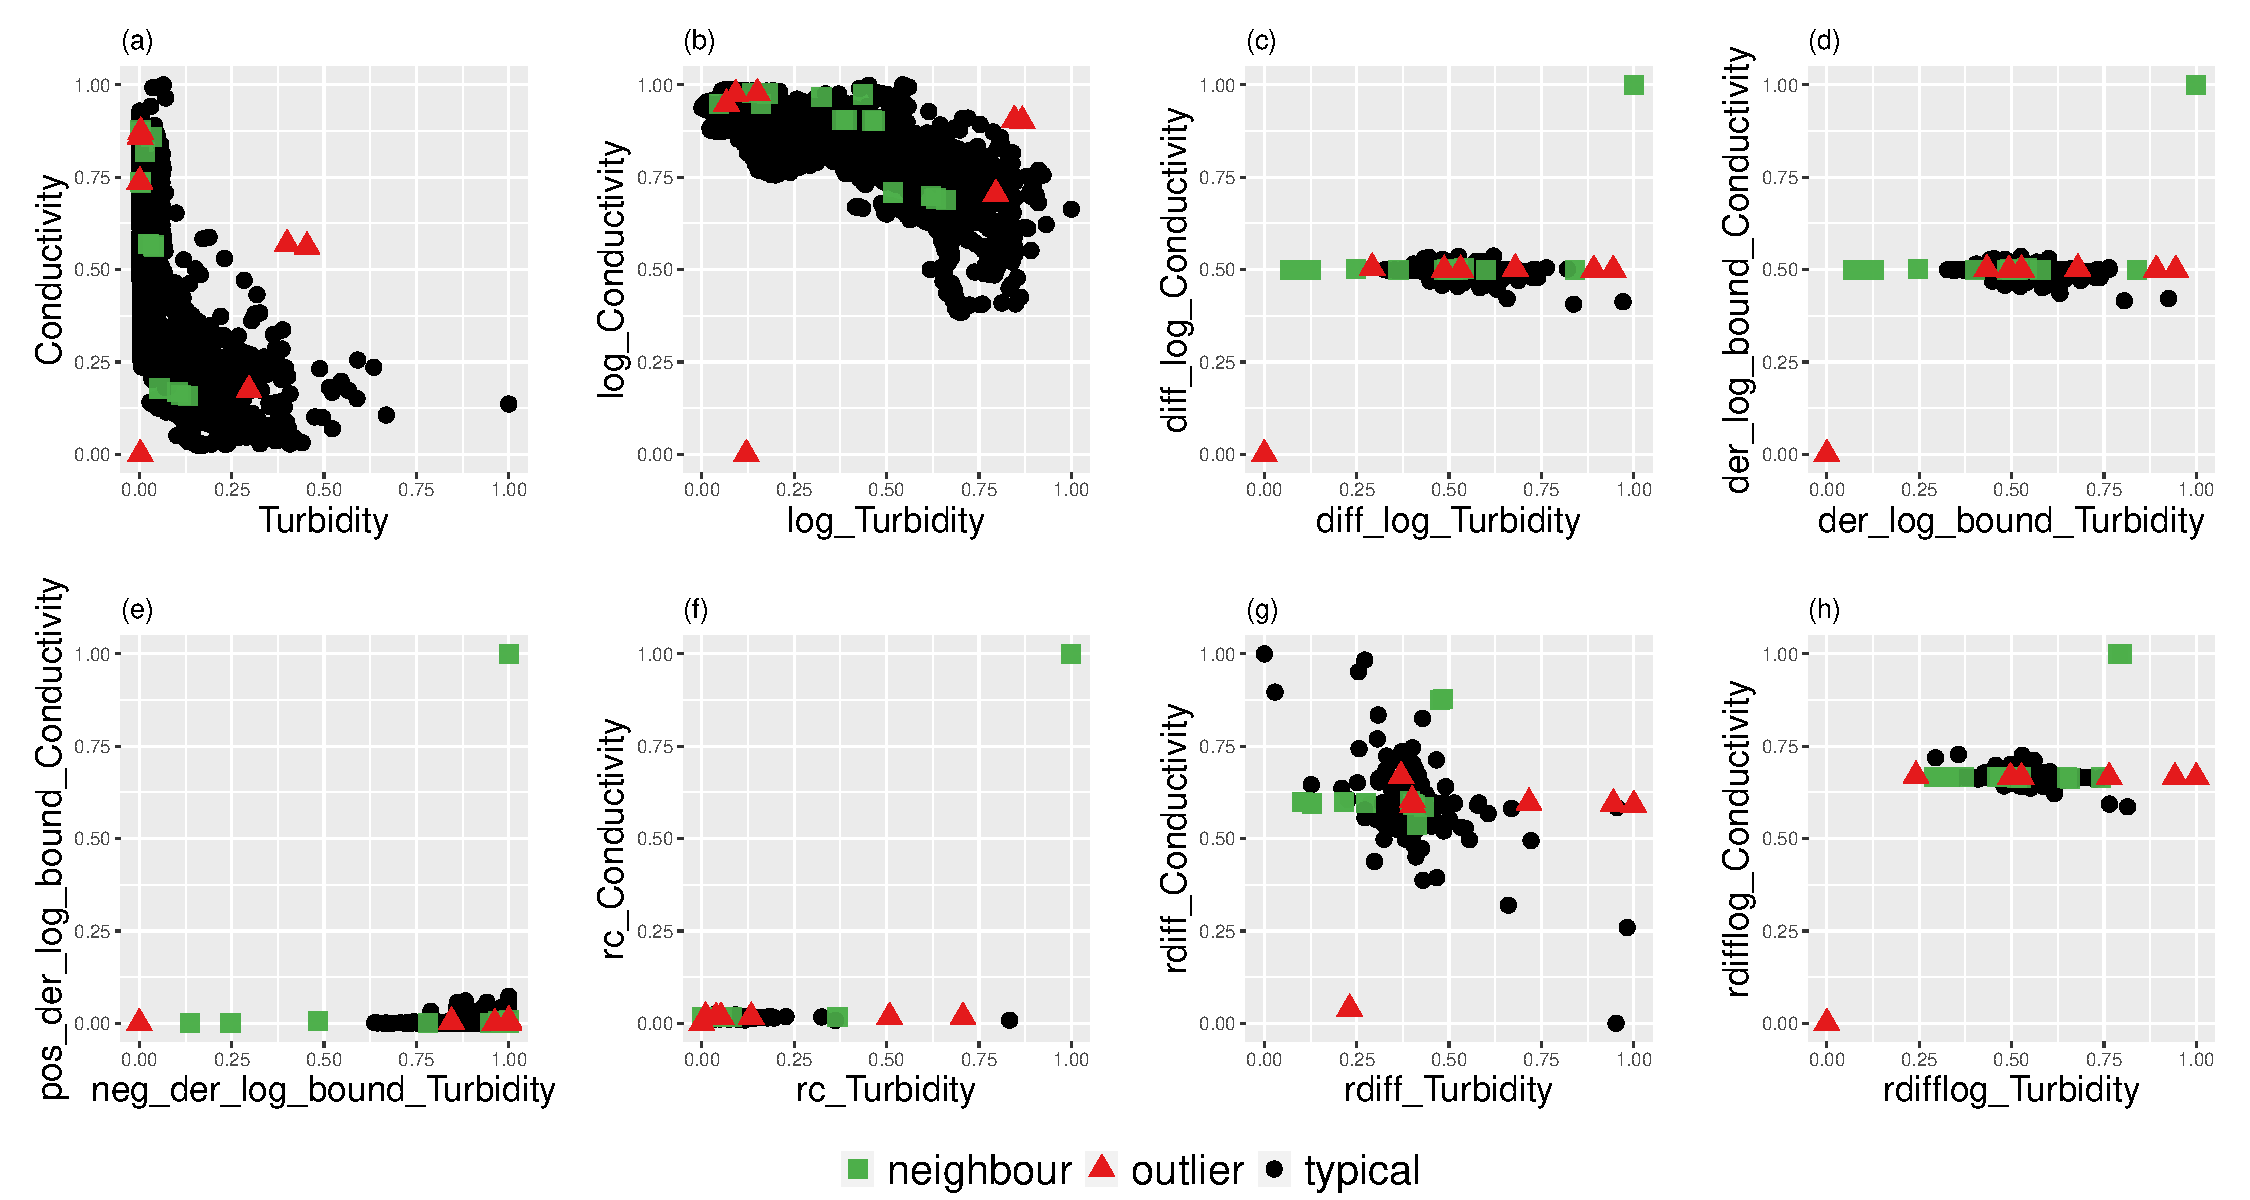
\includegraphics[width=1\linewidth]{./fig/transformType-1.pdf}

}

\caption{Bivariate relationships between transformed series of turbidity and conductivity measured by \textit{in~situ} sensors at Sandy Creek. In each scatter plot, outliers determined by water-quality experts are shown in red, while typical points are shown in black. \color{black} Neighboring points are marked in green. \color{black} (a) Original series, (b) Log transformation, (c) First difference, (d) First derivative, (e) One sided derivative, and (f) Rate of change, (g) Relative difference (for original series), (h) Relative difference (for log transformed series). \color{black}In each scatter plot, data are normalised such that they are bounded by the unit hypercube. \color{black}}\label{fig:transformTypePng}

\end{figure}

\subsection{Calculate outlier scores}\label{sec:outscore}

We considered eight unsupervised outlier scoring techniques for high
dimensional data, involving nearest neighbor distances or densities of
the observations \color{black} and applied them to the three dimensional data space defined by the three variables: turbidity, conductivity and river level. \color{black} Methods based on \(k\)-nearest neighbor distances
(where \(k \in Z^{+}\)) were the \color{black}  NN-HD algorithm (details of this algorithm, which was inspired by HDoutliers algorithm \citep{wilkinsonvisualizing} are provided in Supporting Information), \color{black}  KNN-AGG and KNN-SUM algorithms
\citep{angiulli2002fast,madsen2018ddoutlier} and Local Distance-based
Outlier Factor (LDOF) algorithm \citep{zhang2009new}, which calculate
the outlier score under the assumption that any outlying point (or
outlying clusters of points) in the data space is (are) isolated;
therefore the outliers are those points having the largest \(k\)-nearest
neighbor distances. In contrast, the density based Local Outlier Factor
(LOF) \citep{breunig2000lof}, Connectivity-based Outlier Factor (COF)
\citep{tang2002enhancing}, Influenced Outlierness (INFLO)
\citep{jin2006ranking} and Robust Kernel-based Outlier Factor (RKOF)
\citep{gao2011rkof} algorithms calculate an outlier score based on
how isolated a point is with respect to its surrounding neighbors, and
therefore the outliers are those points having the lowest densities (see
Supporting Information for detail). Each algorithm assigns outlier scores for all of the
data points in the high dimensional space that described the degree of
outlierness of the individual data points such that outliers are those
points having the largest scores
\citep{kriegel2010outlier,shahid2015characteristics}. This step
allowed us to set a \color{black} data driven threshold (Section
\ref{sec:thresholdcalc}) for the outlier scores, to select the most relevant outliers
\citep{chandola2009anomaly}.
\color{black}

\subsection{Calculate outlier threshold}\label{sec:thresholdcalc}

Following \citet{schwarz2008wind}, \citet{burridge2006additive}
and \citet{wilkinsonvisualizing}, we used extreme value theory (EVT)
to calculate \color{black} a separate outlier threshold  for each set of outlier scores calculated using a given unsupervised outlier scoring technique  (introduced in Section
\ref{sec:outscore}) \color{black} and assign a bivariate label
for each point either as an outlier or typical point. \color{black} Thus, 8 outlier scoring techniques resulted 8 different thresholds for a given dataset. \color{black} The threshold
calculation process started from a subset of data \color{black} containing 50\% \color{black} of
observations with the smallest outlier scores, under the assumption that
this subset contained the outlier scores corresponding to typical data
points and the remaining subset contained the scores corresponding to
the possible candidates for outliers. Following Weissman's spacing
theorem \citep{weissman1978estimation}, the algorithm then fit an
exponential distribution to the upper tail of the outlier scores of the
first subset, and computed the upper \(1-\alpha\) (in this work
\(\alpha\) was set to 0.05) points of the fitted cumulative distribution
function, thereby defining an outlying threshold for the next outlier
score. From the remaining subset the algorithm then selected the point
with the smallest outlier score. If this outlier score exceeded the
cutoff point, all the points in the remaining subset were flagged as
outliers and searching for outliers ceased. Otherwise, the point was
declared as a non-outlier and was added to the subset of the typical
points. The threshold was then updated by including the latest addition.
The searching algorithm continued until an outlier score was found that
exceeded the latest threshold \citep{schwarz2008wind}. We performed
this threshold calculation under the assumption that the distribution of
outlier scores produced by each of the eight unsupervised outlier
scoring techniques for high dimensional data was in the maximum domain
of attraction of the Gumbel distribution which consists of distribution
functions with exponentially decaying tails including the exponential,
gamma, normal and log-normal \citep{embrechts2013modelling}.

\subsection{Performance evaluation}\label{sec:evaluation}

\color{black} In this paper, we focused on high priority outliers, as described in \citet{leigh2019framework}, in which importance ranking of different outlier types was done by taking into account the end-user goals and the potential impact of outliers going undetected. However, it is beyond the scope of this paper to discuss in detail the different types of outliers and their importance ranking. For more detail, we refer the reader to  \citet{leigh2019framework}. \color{black} We performed an experimental evaluation on the accuracy and
computational efficiency of our \color{black} oddwater procedure \color{black} with respect to the
eight outlier scoring techniques, using the different transformations \color{black}(Table \ref{table:table_1}) \color{black}
and different combinations of variables (turbidity, conductivity and
river level). These experimental
combinations were evaluated with respect to common measures for binary
classification based on the values of the confusion matrix which
summarizes the false positives (FP; i.e.~when a typical observation is
misclassified as an outlier), false negatives (FN; i.e.~when an actual
outlier is misclassified as a typical observation), true positives (TP;
i.e.~when an actual outlier is correctly classified), and true negatives
(TN; i.e.~when an observation is correctly classified as a typical
point). \color{black} In this work false positives and false negatives  are equally undesirable as false positives may demand unnecessary and/or expensive actions for corrections and refinement and false negatives greatly reduce confidence in the data and results derived from them. The measures we considered include \color{black} accuracy
(\((TP+TN) / (TP+FP+FN+TN)\)) which explains the overall
effectiveness of a classifier; and geometric-mean (GM = \(\sqrt{TP*TN}\)) which
explains the relative balance of TP and TN of the classifier
\citep{sokolova2009systematic}. According to
\citet{hossin2015review}, these measures are not enough to capture
the poor performance of the classifiers in the presence of imbalanced
datasets where the size of the typical class (positive class) is much
larger than the outlying class (negative class). The datasets obtained
from \emph{in~situ} sensors were highly imbalanced and negatively
dependent (i.e.~containing many more typical observations than
outliers). Therefore, we used three additional measures that are
recommended for imbalanced problems with only two classes (i.e.~typical
and outlying) by \citet{ranawana2006optimized}: the negative
predictive value (\(NPV = TN/(FN+TN)\)) which measures the
probability of a negatively predicted pattern actually being negative;
positive predictive value (\(PPV = TP/(TP+FP)\)) which measures the
probability of a positively predicted pattern actually being positive;
and optimized precision \color{black} (\(OP = P- RI \) where \(P = S_{p}N_{n} + S_{n}N_{p}\); \(RI = |S_{p}-S_{n}|/(S_{p} + S_{n})\); \(S_{p} = TN/(TN+FP); S_{n} = TP/(TP+FN)\) and \(N_{p}\) and \(N_{n}\) represent the proportion of positives (outliers) and negatives (typical) within the  entire dataset) \color{black} which is a combination of accuracy,
sensitivity and specificity metrics \citep{ranawana2006optimized}.

To evaluate the performance of our \color{black} oddwater procedure \color{black} we incorporated additional steps after detecting the outlying time points using the
outlying threshold based on EVT. This was done because the time points
declared as outliers by the outlying threshold could correspond to
either the actual outlying points or to their neighbors. Once the time
points were declared as outliers, the corresponding points in the \color{black}  three \color{black} dimensional space were further investigated by comparing their positions
with respect to the median of the typical points declared by the
\color{black} oddwater procedure. \color{black} This step allowed us to find the most influential
variable for each outlying point. For example, in Figure
\ref{fig:transformTypePng}(e) the isolated point in the first quadrant
is an outlier in the two dimensional space due to the outlying behavior
of the conductivity measurement \color{black} because the deviation of this point from the median happens primarily along the conductivity axis. \color{black} In contrast, the four isolated points
in the third quadrant are outliers due to the outlying behavior of the
turbidity measurement \color{black} because the deviations of the four points from the median happen primarily along the turbidity axis. \color{black}  After detecting the most influential \color{black} variable \color{black}
for each outlying instance \color{black} in the three dimensional space, \color{black}  further investigations were carried out
separately for each individual outlying instance \color{black} with respect to the most influential variable detected,\color{black}  to see whether the
outlying instance was due to a sudden spike or a sudden drop by
comparing the direction of the detected points with respect to the mean
of its two immediate surrounding neighbors and itself. These additional
steps in the \color{black} oddwater procedure \color{black} allowed us to  \color{black} trigger an alarm at the actual outlying point in time \color{black} if the neighboring points were declared as outliers instead of the actual outliers. \color{black} However, we acknowledge that these additional steps select only the most influential variable, not all of the influential variables in the presence of more than one influential variable. The additional steps were incorporated solely to measure the performance of the oddwater procedure. In practice, and because the goal is to trigger an alarm in an occurrence of a technical outlier, it is inconsequential  if the alarm is triggered either at the actual time point or at the immediate neighbouring time points corresponding to the actual outlier. As such, users of the oddwater procedure can ignore these additional steps. \color{black}

Using the outlier threshold, our \color{black} oddwater procedure \color{black} assigns a bivariate
label (either as outlier or typical point) to each observed time point
and thereby creates a vector of predicted class labels. That is, if a
time point is declared as an outlier by \color{black} oddwater procedure, \color{black} then
that could be due to at least one variable in the dataset. We also
declared each time point as an outlier or not based on the labels
assigned by the water quality experts. At a given time point, if at
least one variable was labeled as an outlier by the water quality
experts then the corresponding time point was marked as an outlier and
thereby creating a vector of ground-truth labels. Then the performance
measures were calculated based on these two vectors of ground-truth
labels and predicted class labels. \color{black} Thus, this performance evaluation was done with respect to the algorithm's ability to label a point in time as an outlier or not (i.e., a point in time is an outlier if the observed value for any one or more of the three variables measured at that point in time are outliers). \color{black}

\subsection{Software implementation} \label{sec:rpackage}

The \color{black} oddwater procedure \color{black} was implemented in the open source R package
\texttt{oddwater} \citep{oddwater2018}, which provides a
growing list of transformation and outlier scoring methods for
high dimensional data together with visualization and performance
evaluation techniques. Version 0.6.0 of the package \texttt{oddwater} was used for the
results presented herein and is available from Github \color{black} (https://github.com/pridiltal/oddwater). In addition to the implementations available through \texttt{oddwater} package, \texttt{DDoutlier} package \citep{madsen2018ddoutlier} was also  used for outlier score calculations. \color{black} We measured the computation time (minimum
(\(min_t\)), mean (\(mu_t\)), maximum (\(max_t\)) execution time) using
the \texttt{microbenchmark} package \citep{microbenchmark} for
different combinations of algorithms, transformations and variable
combinations on 28 core Xeon-E5-2680-v4 @ 2.40GHz servers. \color{black} We also developed an R Shiny application (available via \texttt{oddwater} R package) to provide interactive visual analytic tools to gain greater insight into the data and perform preliminary investigations of the relationships between water-quality variables at different sites. Further, we have archived a snapshot of version 0.6.0 of the R package on Zenodo (DOI: 10.5281/zenodo.2890469) along with the code and  datasets used, with the aim of  facilitating reproducibility of the results presented herein. \color{black}

\section{Results}\label{sec:application}

\subsection{Analysis of water-quality data from
\emph{in~situ} sensors at Sandy
Creek}\label{sec:analysis-of-water-quality-data-from-in-situ-sensors-at-sandy-creek}

A negative relationship was clearly visible between the water-quality
variables: turbidity and
conductivity and also between conductivity and river level measured by
\emph{in~situ} sensors at Sandy Creek (Figures \ref{fig:VisualiseOutlierPng} and
\ref{fig:VisualiseOutlierPairsTransDataPng}(a,c)). Further, no clear
separation was observed between the target outliers and the typical
points in the original data space
(Figure~\ref{fig:VisualiseOutlierPairsTransDataPng}(a--c)). However, a
clear separation was apparent between the two sets of points once the
one sided derivative transformation (an appropriate transformation for
unevenly spaced data) was applied to the original series
(Figures~
\ref{fig:VisualiseOutlierPairsTransDataPng}(d--f) and \ref{fig:transDemoTCLpng} ).

KNN-AGG and KNN-SUM algorithms performed on all three water-quality
variables together, and on turbidity and conductivity together using the
one sided derivative transformation, gave the highest OP (0.8329)
and NPV values(0.9996), which are the most recommended
measurements for negatively dependent data  where the focus is more on sensitivity (the proportion of positive
patterns being correctly recognized as being positive) than specificity
\citep{ranawana2006optimized}.

\begin{figure}[H]

{\centering 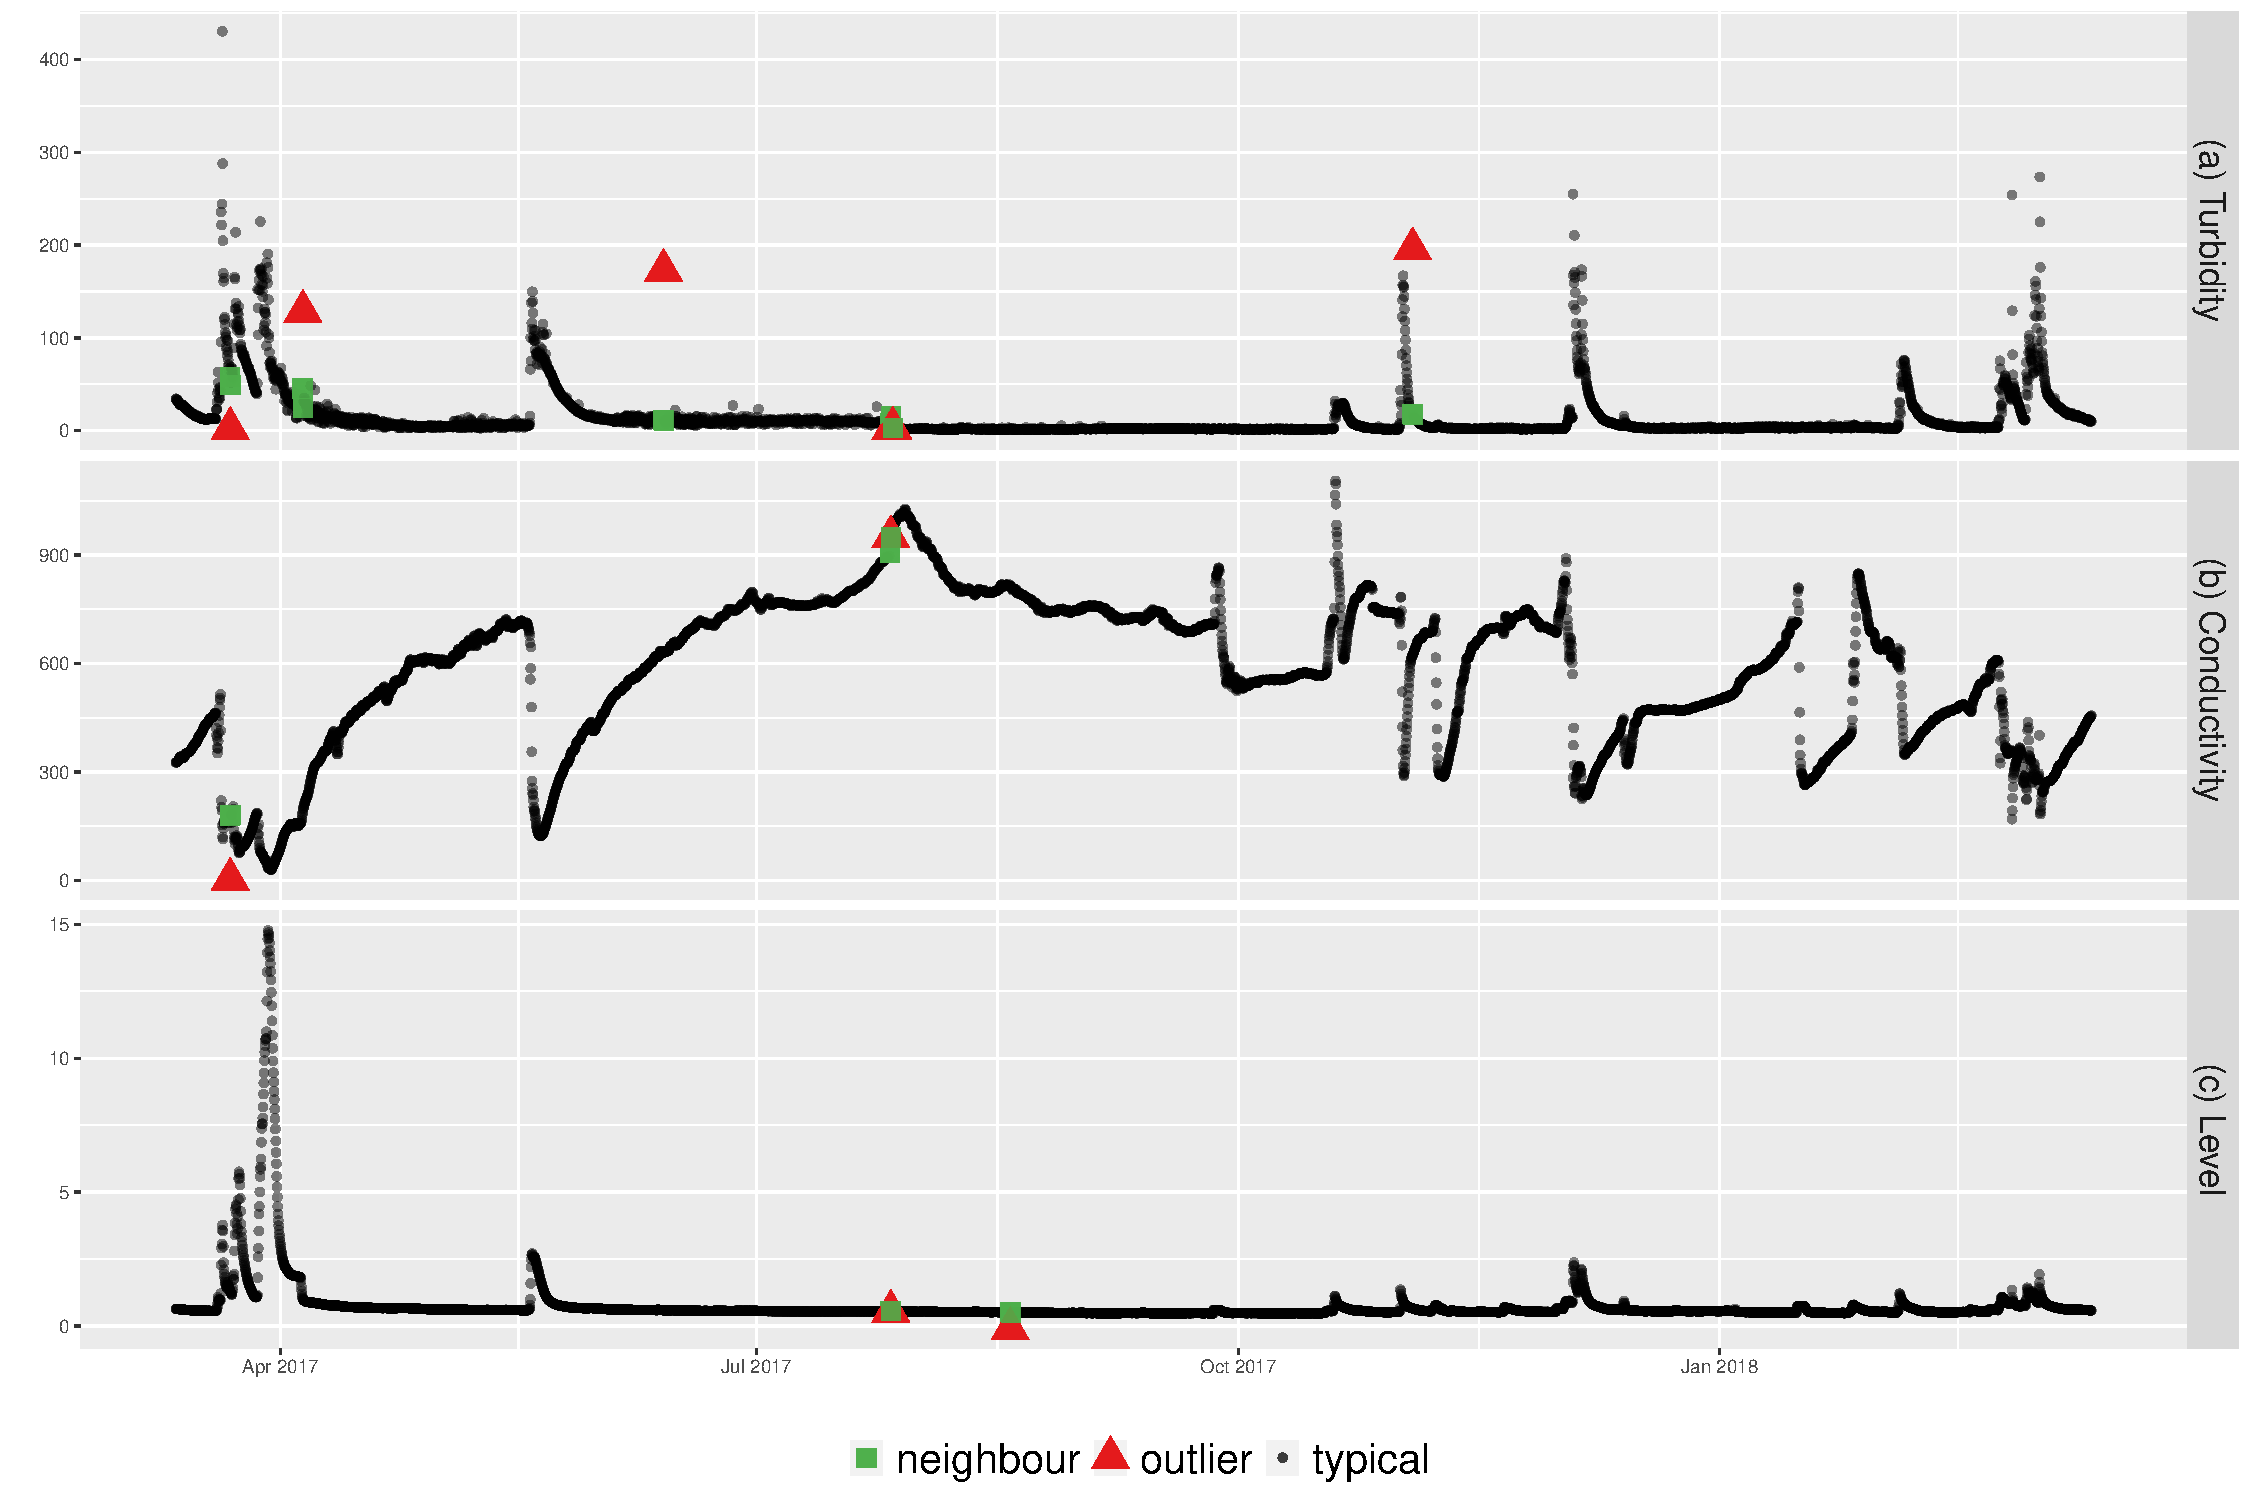
\includegraphics[width=1\textwidth]{./fig/transDemoTCLoriginal-1.pdf}

}

\caption{Time series for turbidity (NTU), conductivity ($\mu$S/cm) and river level (m) measured by \textit{in situ} sensors at Sandy Creek. In each plot, outliers determined by water-quality experts are shown in red. Typical points are shown in black.}\label{fig:VisualiseOutlierPng}
\end{figure}

\begin{figure}[H]

{\centering 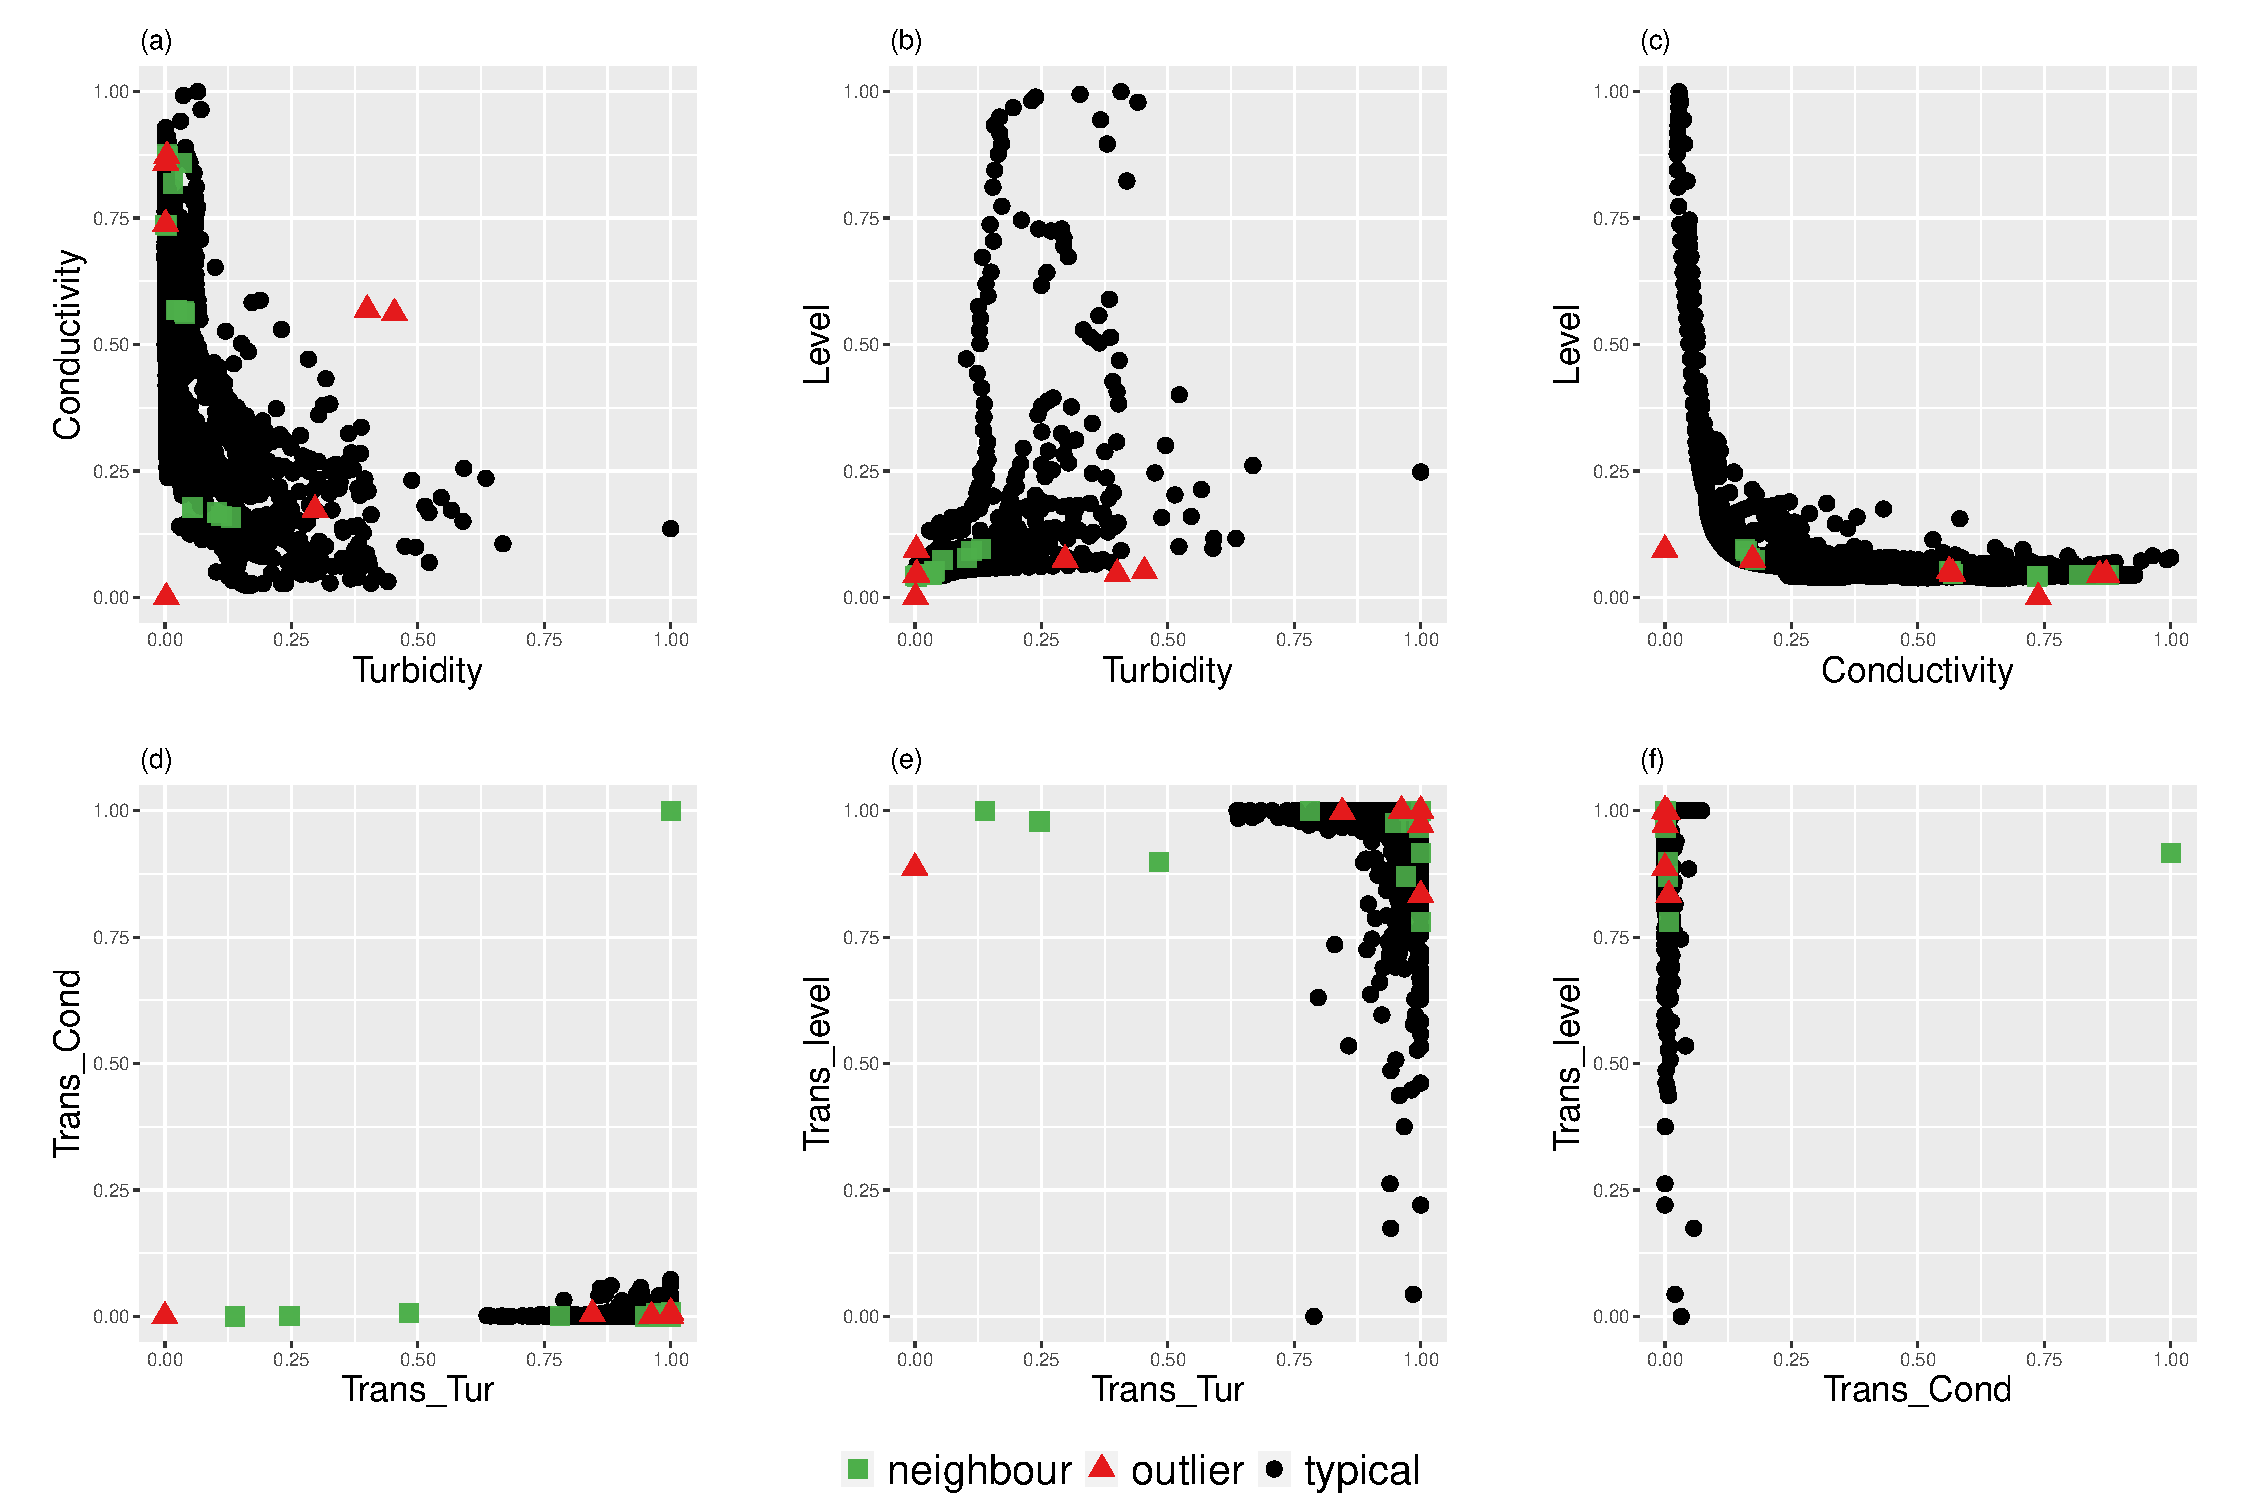
\includegraphics[width=1\textwidth]{./fig/VisualiseOutlierPairsTransData-1.pdf}

}

\caption{Top panel (a--c): Bi-variate relationships between original water-quality variables (turbidity (NTU), conductivity ($\mu$S/cm) and river level (m)) measured by \textit{in situ} sensors at Sandy Creek. Bottom panel (d--f): Bi-variate relationships between transformed series (one sided derivative) of turbidity (NTU), conductivity ($\mu$S/cm) and river level (m) measured by \textit{in situ} sensors at Sandy Creek. In each scatter plot, outliers determined by water-quality experts are shown in red, while typical points are shown in black. Neighboring points are marked in green.}\label{fig:VisualiseOutlierPairsTransDataPng}
\end{figure}

\begin{figure}[H]

{\centering 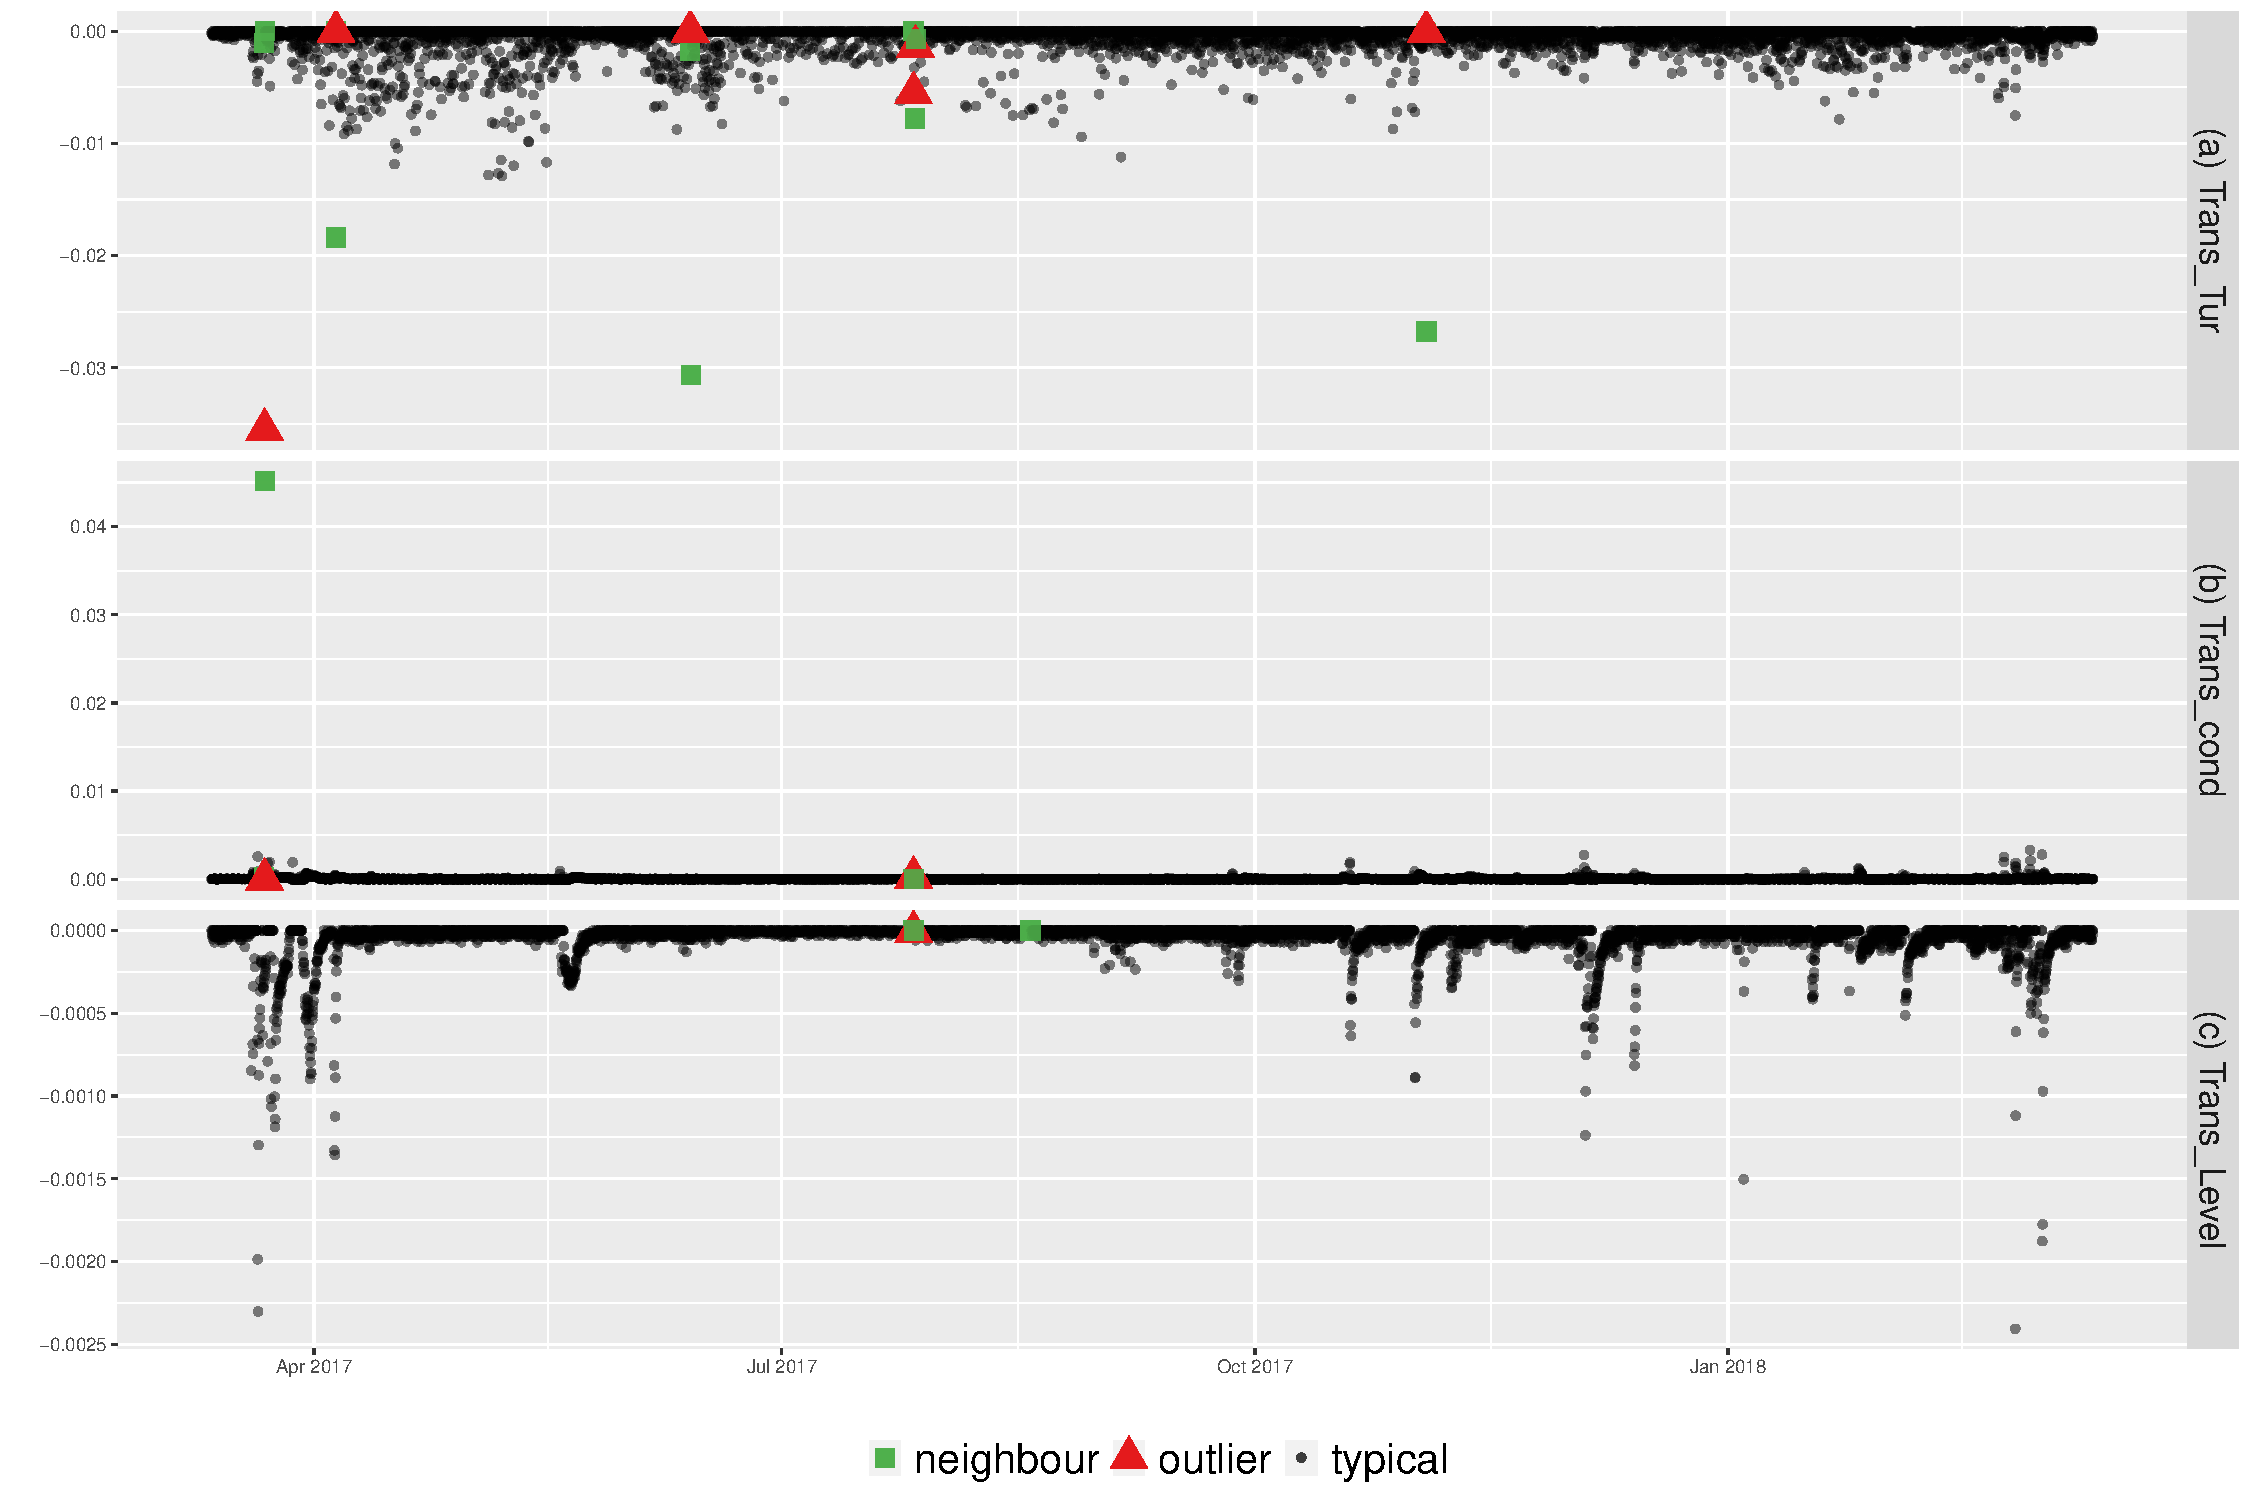
\includegraphics[width=1\textwidth]{./fig/transDemoTCLtrans-1.pdf}
}

\caption{Transformed series (one sided derivatives) of turbidity (NTU), conductivity ($\mu$S/cm) and river level (m) measured by \textit{in situ} sensors at Sandy Creek. In each plot outliers determined by water-quality experts are shown in red, while typical points are shown in black. \color{black} Neighboring points are marked in green \color{black}}\label{fig:transDemoTCLpng}
\end{figure}

\begin{table}[!htbp]
\caption{\label{tab:sandyTable}Performance metrics of outlier
      detection algorithms performed on multivariate water-quality time series
      data (T, turbidity; C, conductivity; L, river level) from in situ sensors at Sandy Creek, arranged in descending
      order of OP values. See Sections 2.7-8 for performance metric codes and details.}
\centering
\resizebox{\linewidth}{!}{
\begin{tabular}{rlllrrrrrrrrrrrr}
\toprule
i & Variables & Transformation & Method & TN & FN & FP & TP & Accuracy & GM & OP & PPV & NPV & min\_t & mu\_t & max\_t\\
\midrule
1 & T-C-L & One sided Derivative & KNN-AGG & 5394 & 2 & 1 & 5 & 0.9994 & 164.23 & 0.83 & 0.83 & 0.9996 & 378.5 & 404.0 & 493.4\\
2 & T-C-L & One sided Derivative & KNN-SUM & 5394 & 2 & 1 & 5 & 0.9994 & 164.23 & 0.83 & 0.83 & 0.9996 & 177.2 & 186.8 & 270.3\\
3 & T-C & First Derivative & \color{black} NN-HD \color{black} & 5393 & 2 & 3 & 4 & 0.9991 & 146.87 & 0.80 & 0.57 & 0.9996 & 40.5 & 45.0 & 72.1\\
4 & T-C & First Derivative & KNN-AGG & 5392 & 2 & 4 & 4 & 0.9989 & 146.86 & 0.80 & 0.50 & 0.9996 & 386.3 & 415.8 & 489.4\\
5 & T-C & One sided Derivative &  \color{black} NN-HD \color{black}  & 5396 & 2 & 0 & 4 & 0.9996 & 146.91 & 0.80 & 1.00 & 0.9996 & 102.7 & 112.9 & 195.4\\
\addlinespace
6 & T-C & One sided Derivative & KNN-AGG & 5395 & 2 & 1 & 4 & 0.9994 & 146.90 & 0.80 & 0.80 & 0.9996 & 381.8 & 411.7 & 518.0\\
7 & T-C & One sided Derivative & KNN-SUM & 5395 & 2 & 1 & 4 & 0.9994 & 146.90 & 0.80 & 0.80 & 0.9996 & 177.9 & 190.4 & 286.2\\
8 & T-C-L & First Derivative & KNN-AGG & 5395 & 4 & 0 & 3 & 0.9993 & 127.22 & 0.60 & 1.00 & 0.9993 & 377.6 & 404.4 & 476.2\\
9 & T-C-L & First Derivative & KNN-SUM & 5395 & 4 & 0 & 3 & 0.9993 & 127.22 & 0.60 & 1.00 & 0.9993 & 179.2 & 188.9 & 273.3\\
10 & T-C & First Derivative & KNN-SUM & 5396 & 4 & 0 & 2 & 0.9993 & 103.88 & 0.50 & 1.00 & 0.9993 & 179.0 & 189.5 & 283.5\\
\addlinespace
11 & T-C & First Derivative & LDOF & 5395 & 4 & 1 & 2 & 0.9991 & 103.87 & 0.50 & 0.67 & 0.9993 & 17261.5 & 17444.7 & 17809.9\\
12 & T-C & One sided Derivative & LDOF & 5395 & 4 & 1 & 2 & 0.9991 & 103.87 & 0.50 & 0.67 & 0.9993 & 17024.3 & 17253.8 & 18079.4\\
13 & T-C-L & First Derivative &  \color{black} NN-HD \color{black}  & 5395 & 5 & 0 & 2 & 0.9991 & 103.87 & 0.44 & 1.00 & 0.9991 & 48.7 & 52.5 & 66.9\\
14 & T-C-L & First Derivative & INFLO & 5381 & 5 & 14 & 2 & 0.9965 & 103.74 & 0.44 & 0.12 & 0.9991 & 1076.5 & 1107.9 & 1168.3\\
15 & T-C-L & First Derivative & COF & 5393 & 5 & 2 & 2 & 0.9987 & 103.86 & 0.44 & 0.50 & 0.9991 & 5869.1 & 5939.8 & 6394.2\\
\addlinespace
16 & T-C-L & First Derivative & RKOF & 5380 & 5 & 15 & 2 & 0.9963 & 103.73 & 0.44 & 0.12 & 0.9991 & 341.6 & 369.7 & 456.1\\
17 & T-C-L & One sided Derivative &  \color{black} NN-HD \color{black}  & 5395 & 5 & 0 & 2 & 0.9991 & 103.87 & 0.44 & 1.00 & 0.9991 & 110.4 & 118.2 & 193.2\\
18 & T-C-L & One sided Derivative & INFLO & 5392 & 5 & 3 & 2 & 0.9985 & 103.85 & 0.44 & 0.40 & 0.9991 & 1071.5 & 1113.6 & 1177.6\\
19 & T-C-L & One sided Derivative & COF & 5393 & 5 & 2 & 2 & 0.9987 & 103.86 & 0.44 & 0.50 & 0.9991 & 5676.8 & 5787.4 & 6238.4\\
20 & T-C-L & One sided Derivative & LDOF & 5392 & 5 & 3 & 2 & 0.9985 & 103.85 & 0.44 & 0.40 & 0.9991 & 17181.5 & 17261.9 & 17435.8\\
\addlinespace
21 & T-C-L & One sided Derivative & LOF & 5392 & 5 & 3 & 2 & 0.9985 & 103.85 & 0.44 & 0.40 & 0.9991 & 500.2 & 516.9 & 596.9\\
22 & T-C-L & One sided Derivative & RKOF & 5387 & 5 & 8 & 2 & 0.9976 & 103.80 & 0.44 & 0.20 & 0.9991 & 338.9 & 370.5 & 464.0\\
23 & T-C-L & Original series & KNN-AGG & 5394 & 5 & 1 & 2 & 0.9989 & 103.87 & 0.44 & 0.67 & 0.9991 & 376.6 & 391.6 & 465.3\\
24 & T-C-L & Original series & INFLO & 5386 & 5 & 9 & 2 & 0.9974 & 103.79 & 0.44 & 0.18 & 0.9991 & 1034.3 & 1070.7 & 1136.7\\
25 & T-C-L & Original series & LDOF & 5393 & 5 & 2 & 2 & 0.9987 & 103.86 & 0.44 & 0.50 & 0.9991 & 17078.5 & 17156.9 & 17308.1\\
\addlinespace
26 & T-C-L & Original series & RKOF & 5392 & 5 & 3 & 2 & 0.9985 & 103.85 & 0.44 & 0.40 & 0.9991 & 322.3 & 354.0 & 426.4\\
27 & T-C & First Derivative & INFLO & 5392 & 5 & 4 & 1 & 0.9983 & 73.43 & 0.28 & 0.20 & 0.9991 & 1134.6 & 1194.9 & 1271.1\\
28 & T-C & First Derivative & COF & 5396 & 5 & 0 & 1 & 0.9991 & 73.46 & 0.28 & 1.00 & 0.9991 & 5881.5 & 5991.8 & 6552.4\\
29 & T-C & First Derivative & LOF & 5394 & 5 & 2 & 1 & 0.9987 & 73.44 & 0.28 & 0.33 & 0.9991 & 498.3 & 512.3 & 596.1\\
30 & T-C & First Derivative & RKOF & 5392 & 5 & 4 & 1 & 0.9983 & 73.43 & 0.28 & 0.20 & 0.9991 & 335.1 & 363.2 & 435.7\\
\addlinespace
31 & T-C & One sided Derivative & INFLO & 5394 & 5 & 2 & 1 & 0.9987 & 73.44 & 0.28 & 0.33 & 0.9991 & 1153.1 & 1207.0 & 1281.9\\
32 & T-C & One sided Derivative & COF & 5394 & 5 & 2 & 1 & 0.9987 & 73.44 & 0.28 & 0.33 & 0.9991 & 5755.0 & 5880.8 & 6420.8\\
33 & T-C & One sided Derivative & LOF & 5384 & 5 & 12 & 1 & 0.9969 & 73.38 & 0.28 & 0.08 & 0.9991 & 501.1 & 511.3 & 585.7\\
34 & T-C & One sided Derivative & RKOF & 5380 & 5 & 16 & 1 & 0.9961 & 73.35 & 0.28 & 0.06 & 0.9991 & 339.5 & 368.3 & 456.6\\
35 & T-C & Original series & KNN-AGG & 5395 & 5 & 1 & 1 & 0.9989 & 73.45 & 0.28 & 0.50 & 0.9991 & 371.5 & 405.1 & 483.7\\
\addlinespace
36 & T-C & Original series & INFLO & 5387 & 5 & 9 & 1 & 0.9974 & 73.40 & 0.28 & 0.10 & 0.9991 & 1095.2 & 1143.6 & 1219.4\\
37 & T-C & Original series & LDOF & 5394 & 5 & 2 & 1 & 0.9987 & 73.44 & 0.28 & 0.33 & 0.9991 & 16842.1 & 17022.9 & 17414.4\\
38 & T-C & Original series & RKOF & 5393 & 5 & 3 & 1 & 0.9985 & 73.44 & 0.28 & 0.25 & 0.9991 & 321.0 & 351.8 & 440.3\\
39 & T-C-L & First Derivative & LDOF & 5395 & 6 & 0 & 1 & 0.9989 & 73.45 & 0.25 & 1.00 & 0.9989 & 17253.9 & 17323.2 & 17400.9\\
40 & T-C-L & First Derivative & LOF & 5395 & 6 & 0 & 1 & 0.9989 & 73.45 & 0.25 & 1.00 & 0.9989 & 504.6 & 517.1 & 604.4\\
\addlinespace
41 & T-C-L & Original series &  \color{black} NN-HD \color{black}  & 5394 & 6 & 1 & 1 & 0.9987 & 73.44 & 0.25 & 0.50 & 0.9989 & 45.4 & 48.6 & 60.3\\
42 & T-C-L & Original series & KNN-SUM & 5395 & 6 & 0 & 1 & 0.9989 & 73.45 & 0.25 & 1.00 & 0.9989 & 164.7 & 177.3 & 243.4\\
43 & T-C-L & Original series & COF & 5395 & 6 & 0 & 1 & 0.9989 & 73.45 & 0.25 & 1.00 & 0.9989 & 5864.4 & 5931.7 & 6329.7\\
44 & T-C-L & Original series & LOF & 5395 & 6 & 0 & 1 & 0.9989 & 73.45 & 0.25 & 1.00 & 0.9989 & 480.2 & 505.0 & 576.2\\
45 & T-C & Original series &  \color{black} NN-HD \color{black}  & 5395 & 6 & 1 & 0 & 0.9987 & 0.00 & 0.00 & 0.00 & 0.9989 & 38.1 & 41.7 & 66.3\\
\addlinespace
46 & T-C & Original series & KNN-SUM & 5396 & 6 & 0 & 0 & 0.9989 & 0.00 & 0.00 & NaN & 0.9989 & 172.7 & 184.6 & 272.5\\
47 & T-C & Original series & COF & 5396 & 6 & 0 & 0 & 0.9989 & 0.00 & 0.00 & NaN & 0.9989 & 5826.3 & 5896.4 & 6804.3\\
48 & T-C & Original series & LOF & 5396 & 6 & 0 & 0 & 0.9989 & 0.00 & 0.00 & NaN & 0.9989 & 477.0 & 502.7 & 568.0\\
\bottomrule
\end{tabular}}
\end{table}

Based on OP values, the one sided derivative transformation outperformed
the first derivative transformation (Table \ref{tab:sandyTable}, rows
1--5 compared to rows 6--10). Further, the distance-based outlier detection
algorithms \color{black} NN-HD \color{black}, KNN-AGG and KNN-SUM outperformed all others
(Table \ref{tab:sandyTable}, rows 1--10 compared to rows 11--48). Among
the three methods the performance of \(k\)-nearest neighbor
distance-based algorithms were only slightly higher (OP = 0.8329) than
the \color{black} NN-HD \color{black} algorithm (OP= 0.7996), which is based only on the
nearest neighbor distance. The algorithm combinations with the five
highest OP values also had high PPV (approximately 0.8). Furthermore,
considering river level for the detection of outliers in the
water-quality sensors slightly improved the performance
(OP = 0.8329). Among the analysis with transformed series, LOF with
the first derivative transformation performed the least well
(OP= 0.2489). \color{black} For most of the outlier \color{black} detection algorithms
(KNN-SUM, KNN-AGG, \color{black} NN-HD \color{black}, COF, LOF and INFLO) the poorest
performances were associated with the untransformed original series,
having the lowest OP and NPV values, highlighting how data
transformation can improve the ability of outlier detection algorithms
while maintaining low false detection rates.

\begin{figure}[H]

{\centering 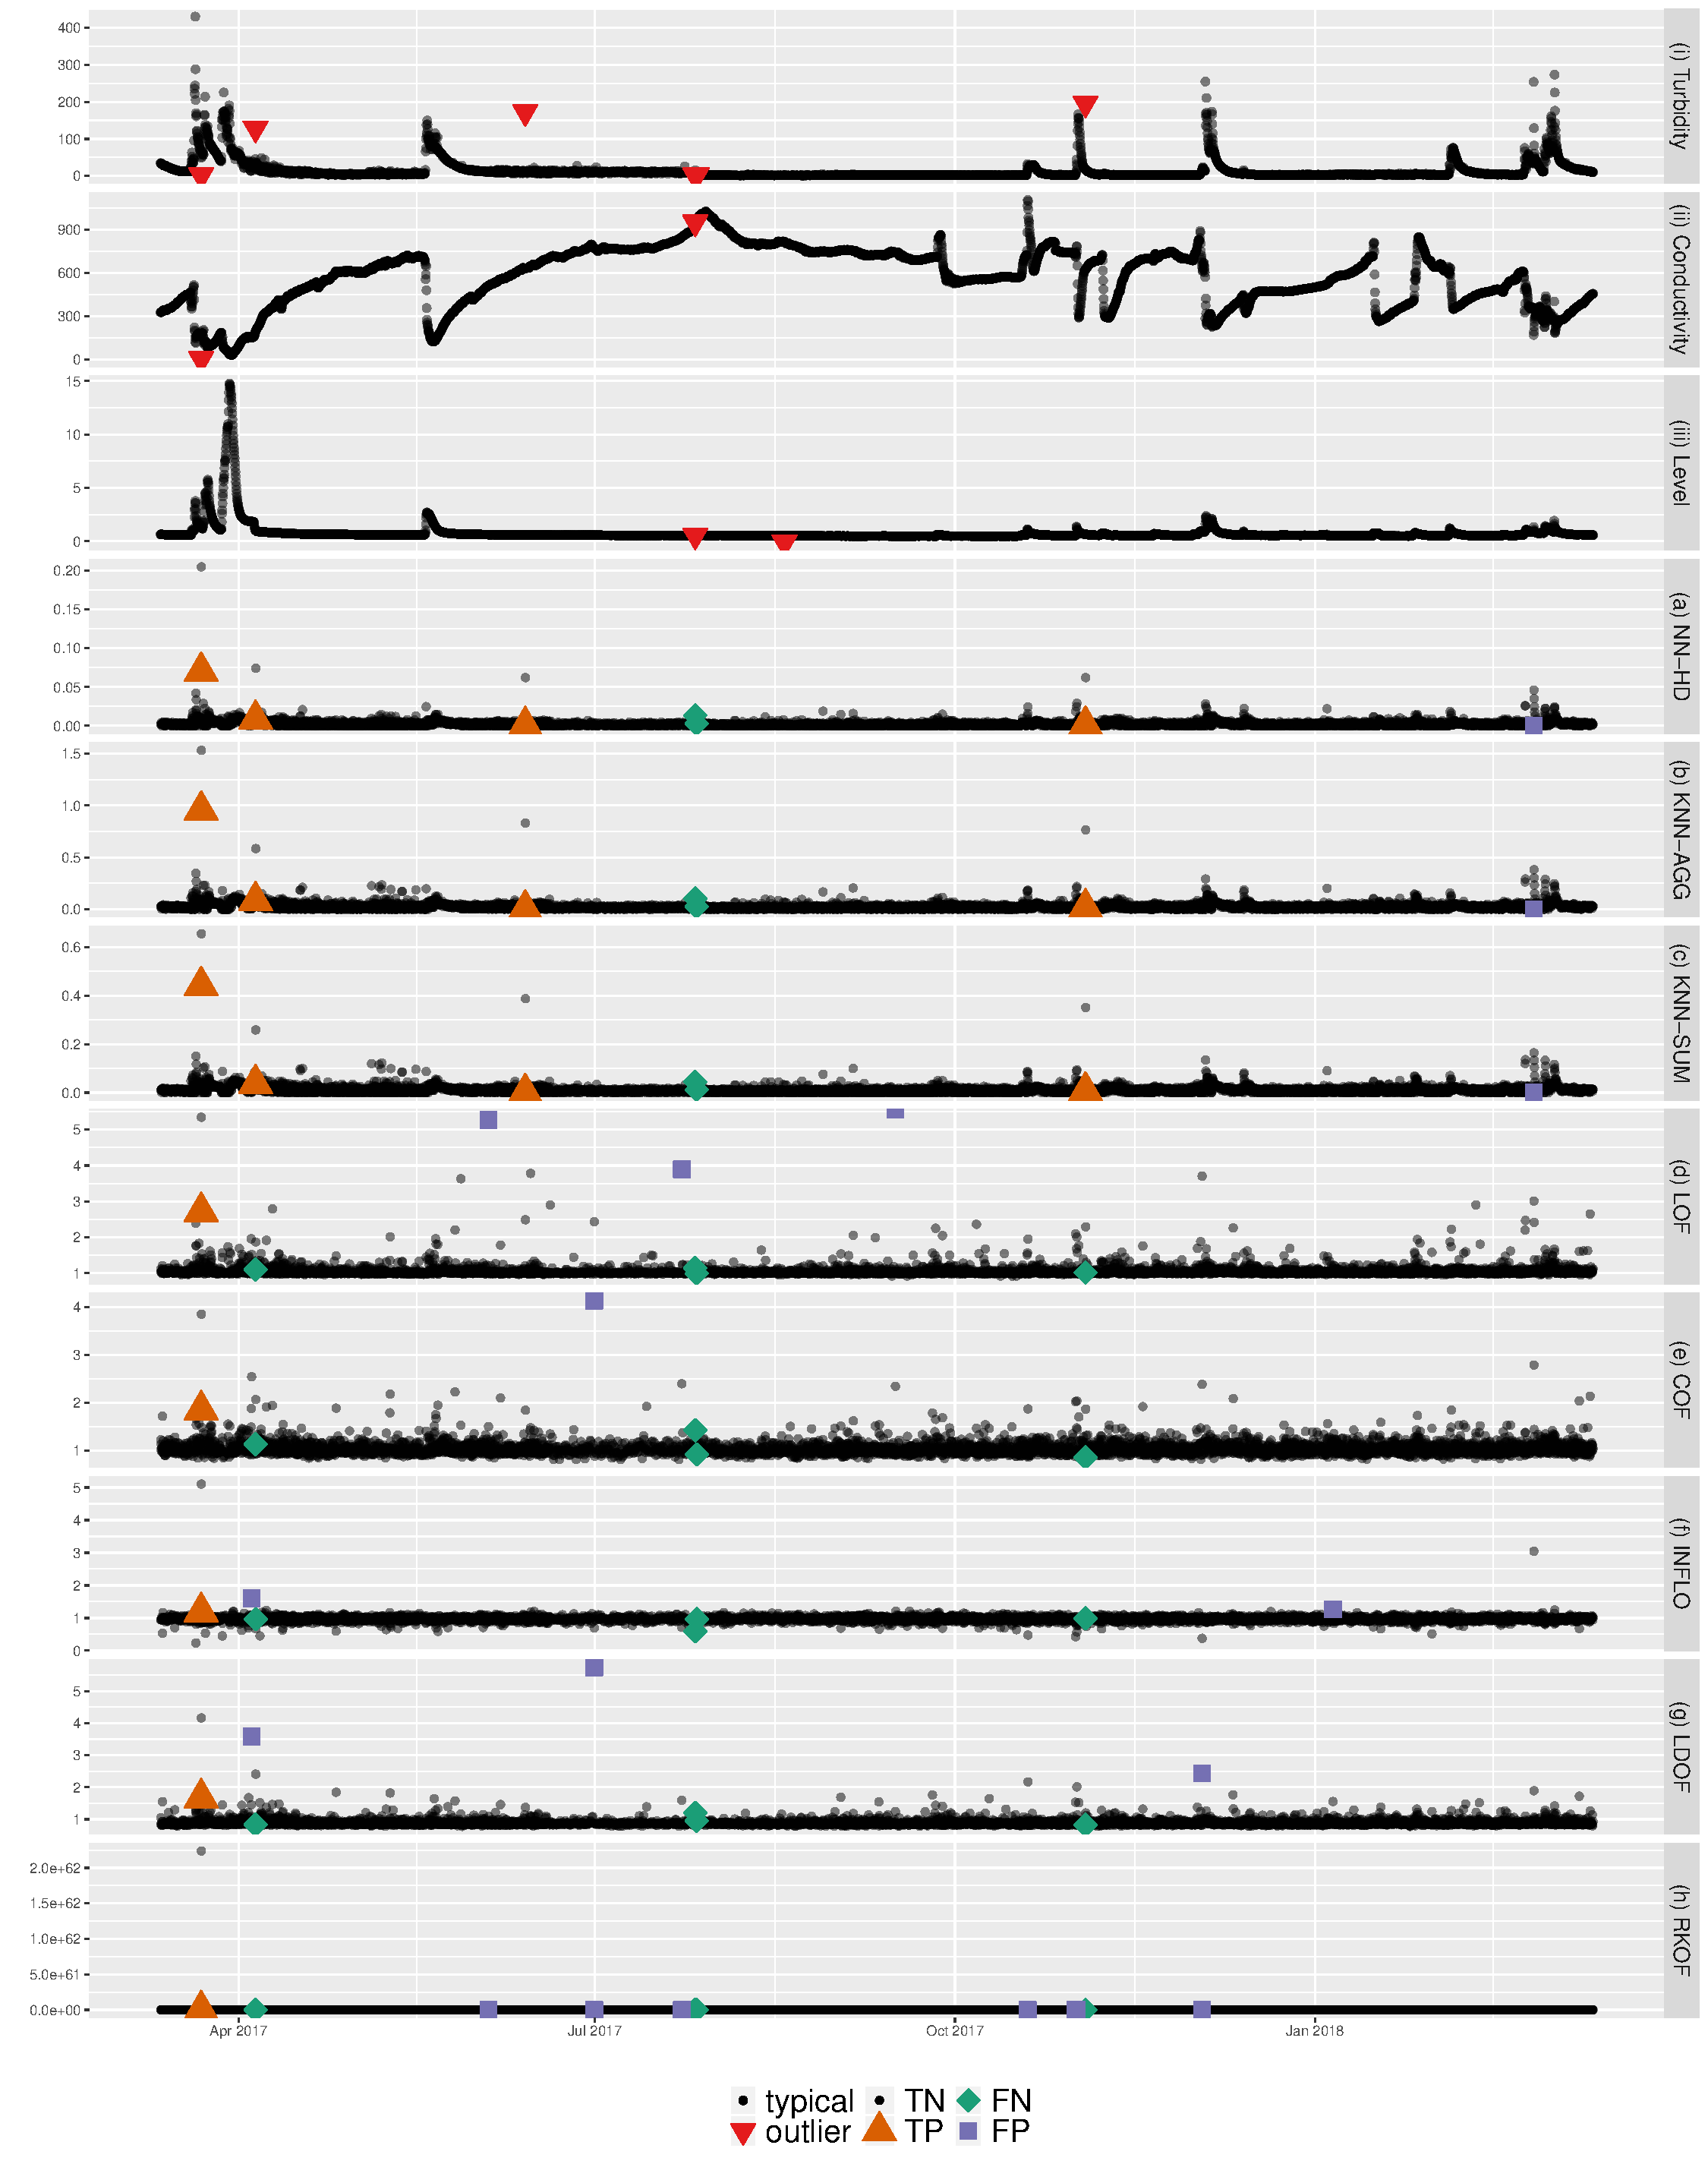
\includegraphics[width=1\linewidth,height=0.8\textheight]{./fig/onesidedderivativeTCLsandy-1.pdf}

}
\caption{Classification of outlier scores produced from different algorithms as true negatives (TN), true positives (TP), false negatives (FN), false positives (FP). The top three panels (i, ii, iii) correspond to the original series (turbidity, conductivity and river level) measured by \textit{in situ} sensors at Sandy Creek. The target outliers (detected by water-quality experts) are shown in red, while typical points are shown in black. The remaining panels (a--h) give outlier scores produced by different outlier detection algorithms for high dimensional data when applied to the transformed series (one sided derivative) of the three variables: turbidity, conductivity and level. \color{black} Through different outlier scoring algorithms (Panel a - h) we are evaluating whether each point in time is an outlier or not. Therefore, from Panel a-h, if the outlier scoring algorithm is effective, then there should be either TP or TN  at each point in time when either a red triangle is plotted in at least one of the three panels (i- iii), or  black dots are plotted  in all of the top three panels (i - iii), respectively. Since outlier scores are non negative and are mostly clustered near zero, with some occasional high values, a square root transformation was applied to reduce skewness of the data in Panel (a) to (h). \color{black}}\label{fig:osDevTCLSandy}
\end{figure}

The three outlier detection algorithms that demonstrated the highest
level of accuracy (\color{black} NN-HD, \color{black} KNN-AGG and KNN-SUM) also outperformed
the others with respect to computational time. \color{black} NN-HD \color{black} algorithm
required the least computational time. Among the remaining two, the mean
computational time of KNN-AGG (\(\approx\) 400 milliseconds) was twice
that of KNN-SUM's (\(< 200\) milliseconds). LOF and its extensions
(INFLO, COF and LDOF) demonstrated the poorest performance with respect
computational time (\(> 500\) milliseconds on average).

Only KNN-SUM and KNN-AGG assigned high scores to most of the targeted
outliers in turbidity, conductivity and level data transformed using the
one-sided derivative (Figure \ref{fig:osDevTCLSandy}(a,b)). For each
outlying instance however, the next immediate neighboring point was
assigned the high outlier score instead of the true outlying point.
After determining the most influential variable using the additional steps of the algorithm (Section \ref{sec:evaluation}), adjustments were made to correct this to the actual outlier. The outlier scores produced by
LOF and COF (Figure \ref{fig:osDevTCLSandy}(d,f)) were unable to capture
the outlying behaviors correctly and demonstrated high scattering. \color{black} In comparison to other outlier  scoring  algorithms, KNN-SUM
algorithm displayed a good compromise between
 accuracy and computational efficiency
 ( Table \ref{tab:sandyTable}).\color{black}

\subsection{Analysis of water-quality data from
\emph{in~situ} sensors at Pioneer
River}\label{analysis-of-water-quality-data-from-in-situ-sensors-at-pioneer-river}

Some of the target outliers in the data obtained from the \emph{in situ}
sensors at Pioneer River only deviated slightly from the general trend
(Figure \ref{fig:VisualiseOutlierPioneerpng}), making outlier detection
challenging. A negative relationship was clearly visible between
turbidity and conductivity (Figure
\ref{fig:VisualiseOutlierPairstransDataPioneerPng}(a)), however the
relationship between level and conductivity was complex (Figure
\ref{fig:VisualiseOutlierPairstransDataPioneerPng}(c)). Most of the
target outliers were masked by the typical points in the original space
(Figure \ref{fig:VisualiseOutlierPairstransDataPioneerPng}(a--c)).
Similar to Sandy Creek, data obtained from the sensors at Pioneer River
showed good separation between outliers and typical points under the one
sided derivative transformation (Figures~
\ref{fig:VisualiseOutlierPairstransDataPioneerPng}(d--f) and \ref{fig:transdemoTCLpioneerPng}). However,
the sudden spikes in turbidity labeled as outliers by water-quality
experts could not be separated from the majority by a large distance and
were only visible as a small group (micro cluster
\citep{goldstein2016comparative}) in the boundary defined by the
typical points (Figure
\ref{fig:VisualiseOutlierPairstransDataPioneerPng}(d, e)).

From the performance analysis it was observed that turbidity and
conductivity together produced better results (Table
\ref{tab:pioneerTable}, rows 1--3) than when combined with river level, which
tended to reduce the performance (i.e. generating lower OP and NPV values) while increasing the
false negative rate (Table \ref{tab:pioneerTable}, rows 4--5). KNN-AGG and
KNN-SUM (Table \ref{tab:pioneerTable}, rows 1--3) had the highest
accuracy (0.9978), lowest error rates (0.0022), highest geometric means (492.8012), highest OP (0.8845) and highest NPV (0.9984). Despite the challenge given by the small spikes which could not be clearly separated from the typical points, KNN-AGG, KNN-SUM and \color{black} NN-HD \color{black} with one sided
derivatives of turbidity and conductivity still detected some of those
points as outliers while maintaining low false negative and false
positive rates. Similar to Sandy Creek, \color{black} NN-HD \color{black} (\textless{} 200
milliseconds on average) and KNN-SUM (\textless{} 230 milliseconds on
average) demonstrated the highest computational efficiency for the data
obtained from Pioneer River.

\begin{figure}[H]

{\centering 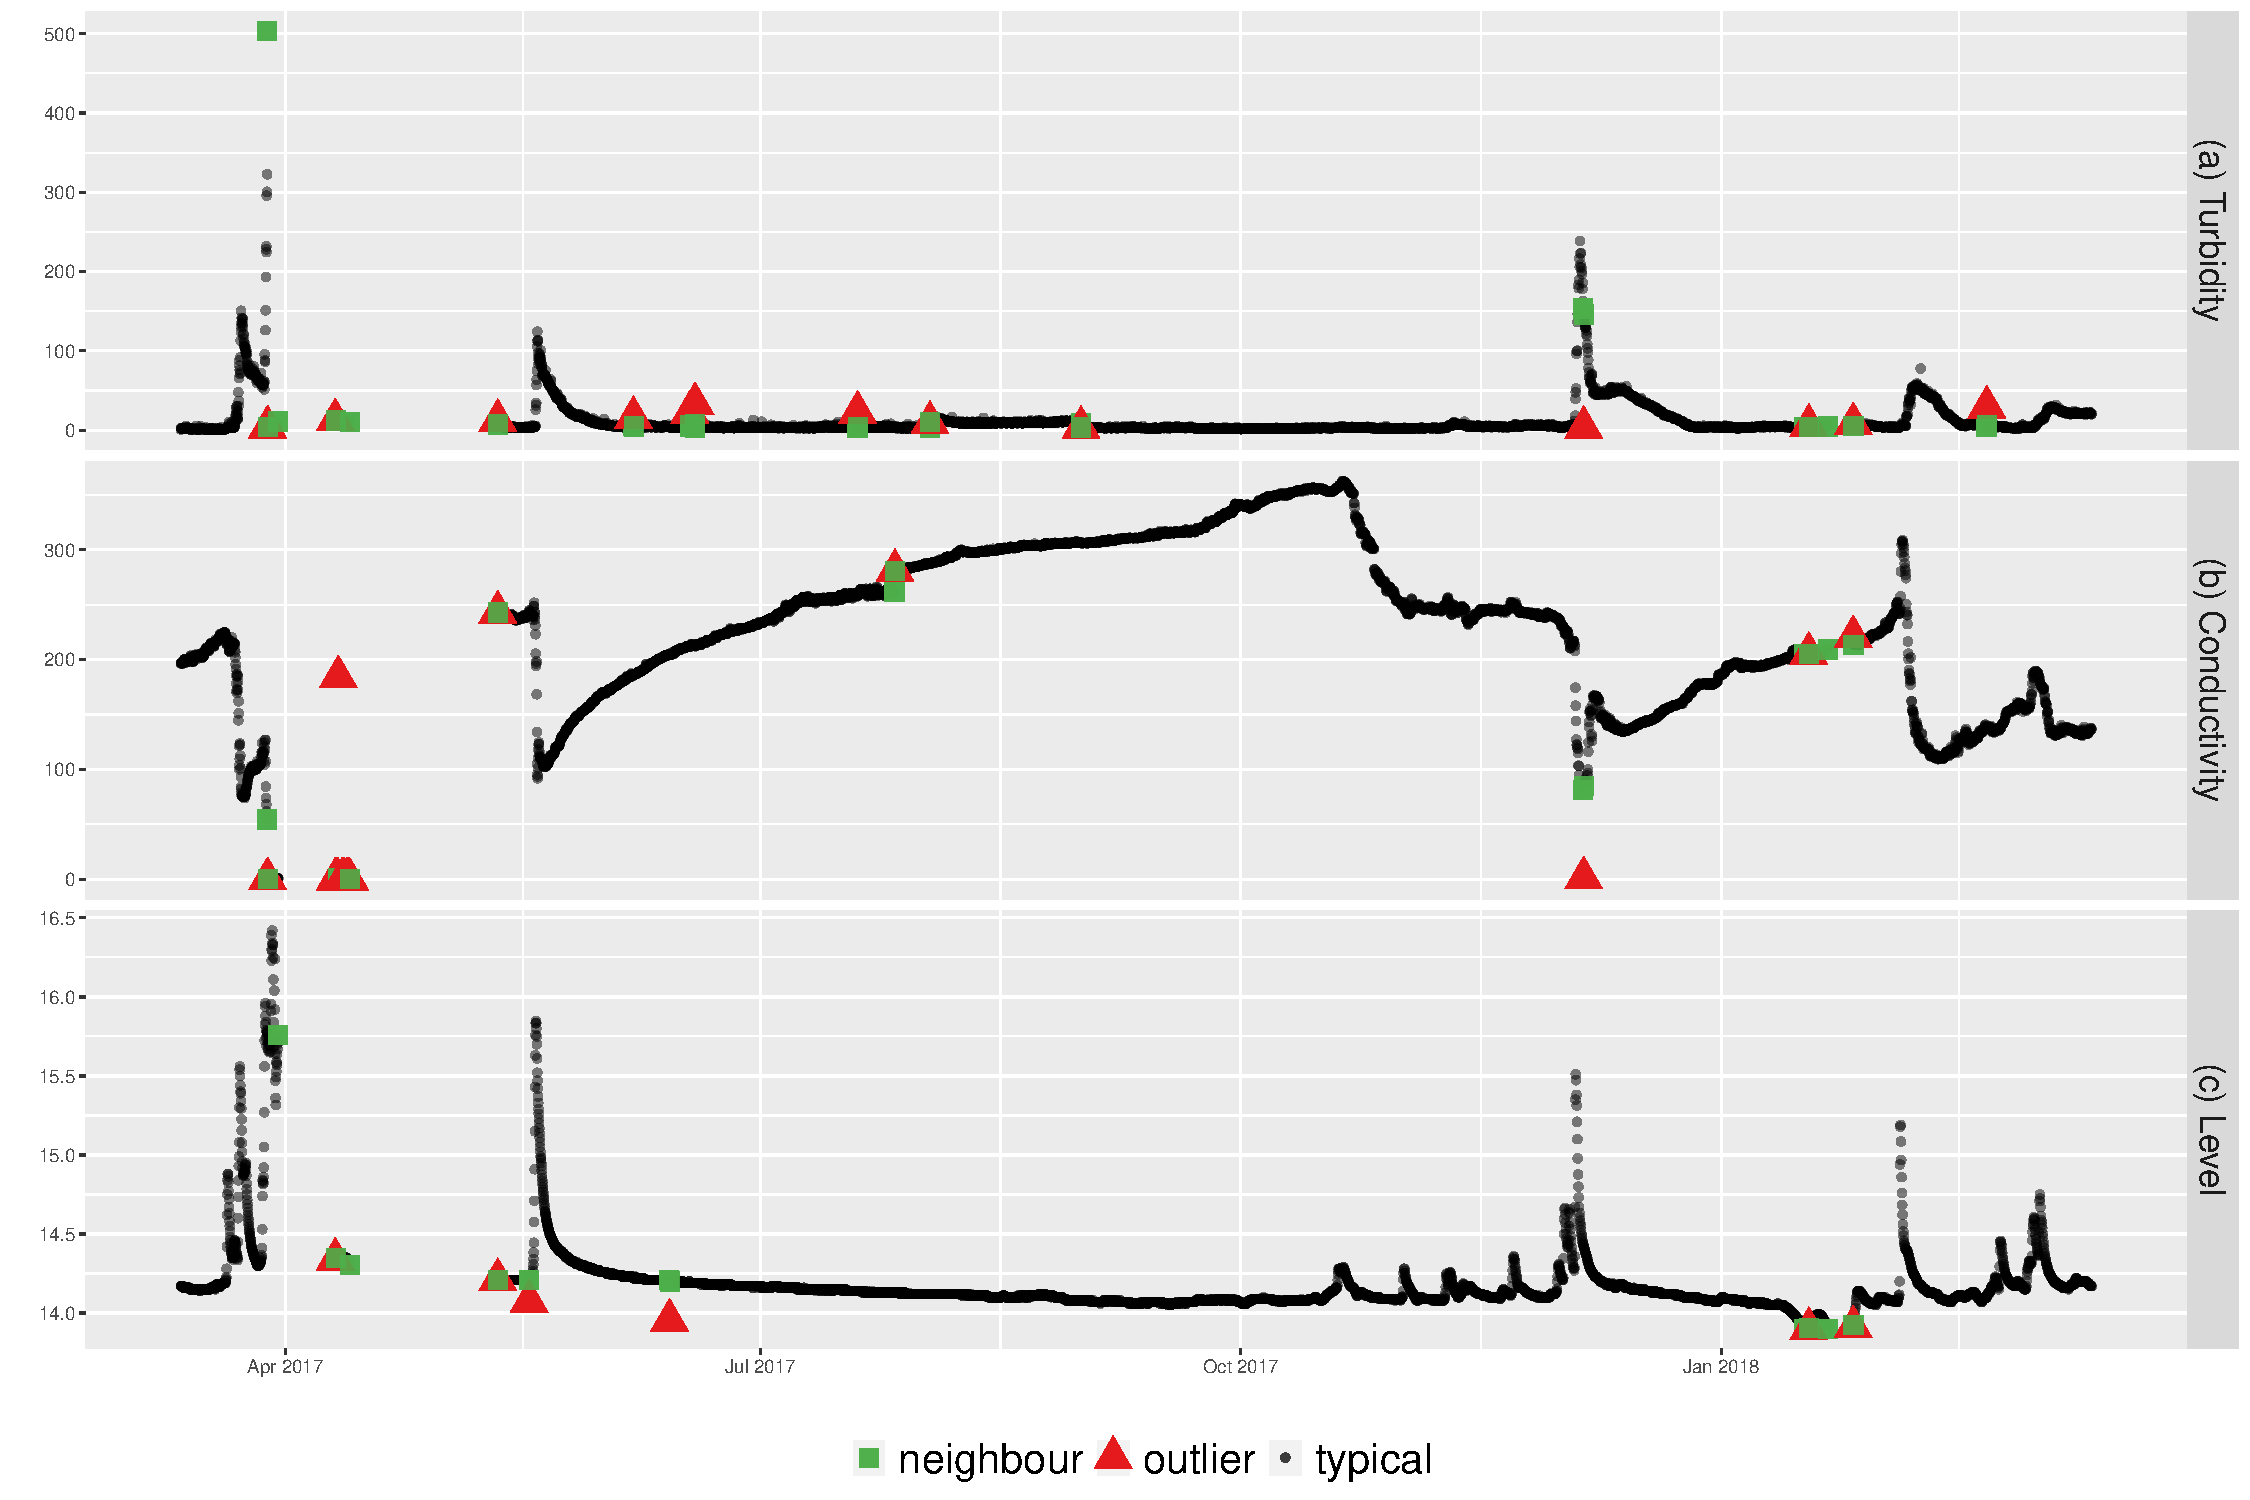
\includegraphics[width=1\textwidth]{./fig/transdemoTCLPioneerOriginal-1.pdf}

}

\caption{Time series for turbidity (NTU), conductivity ($\mu$S/cm) and river level (m) measured by \textit{in situ} sensors at Pioneer River. In each plot, outliers determined by water-quality experts are shown in red, while typical points are shown in black.}\label{fig:VisualiseOutlierPioneerpng}
\end{figure}

\begin{figure}[H]

{\centering 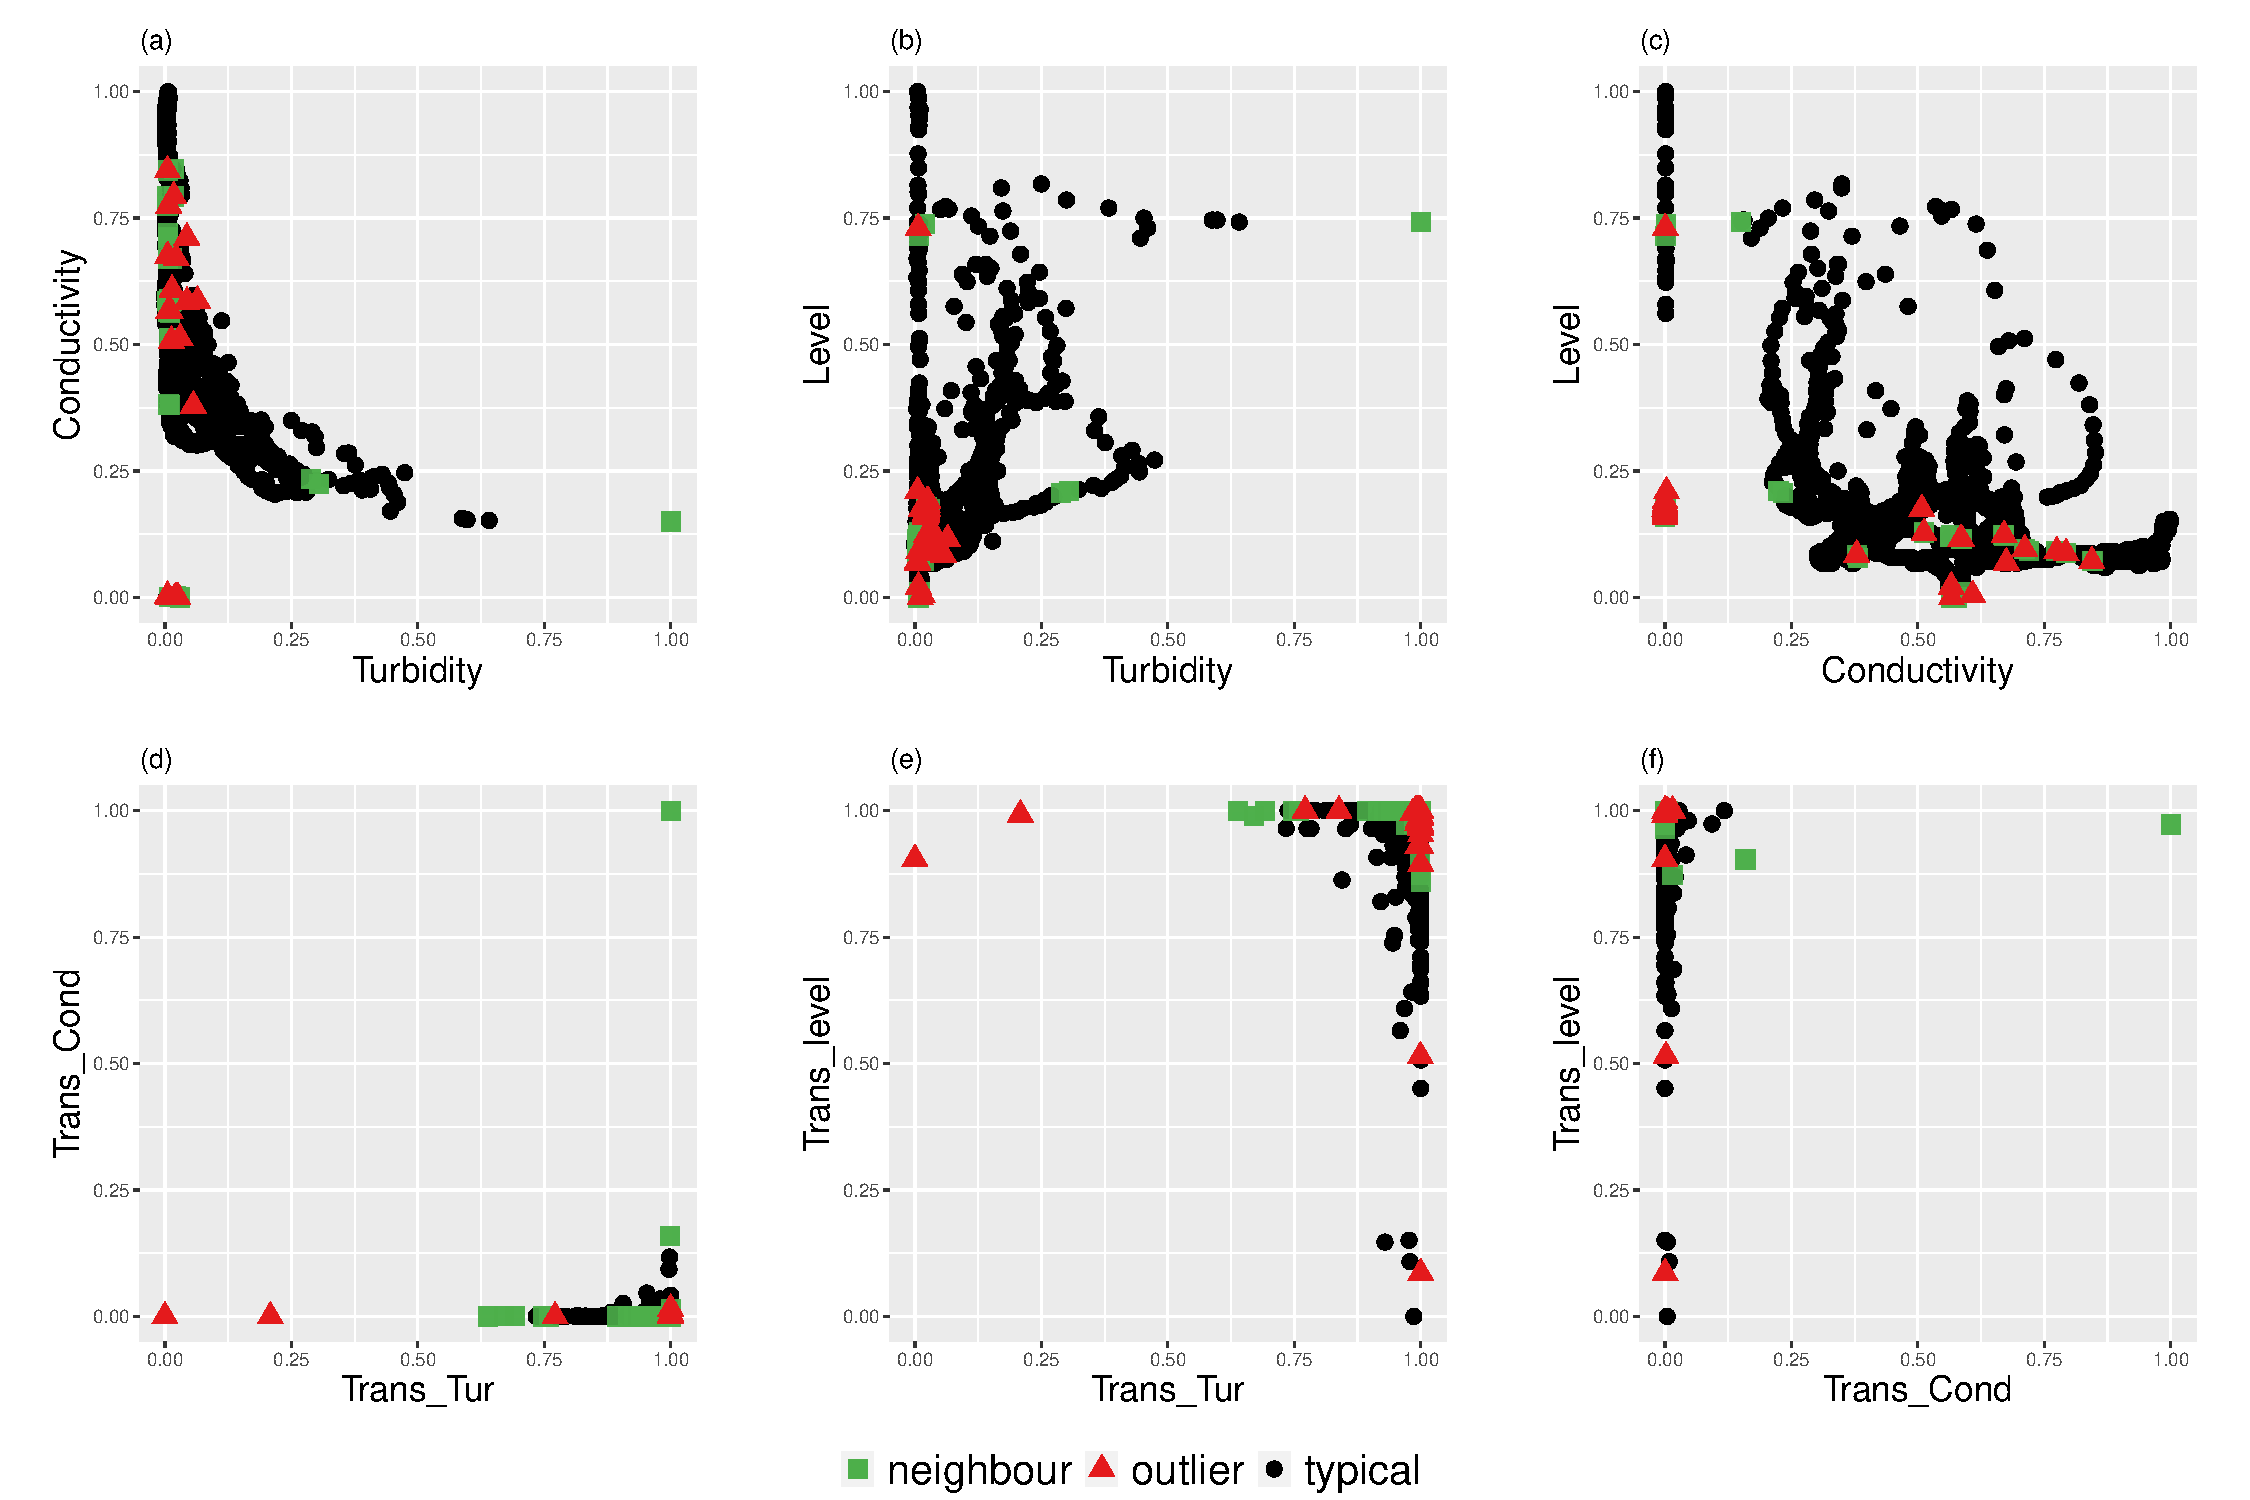
\includegraphics[width=1\textwidth]{./fig/VisualiseOutlierPairsOriginalDataPioneer-1.pdf}

}

\caption{Top panel (a--c): Bi-variate relationships between original water-quality variables (turbidity (NTU), conductivity ($\mu$S/cm) and river level (m)) measured by \textit{in situ} sensors at Pioneer River. Bottom panel (d--f): Bi-variate relationships between transformed series (one sided derivative) of turbidity (NTU), conductivity ($\mu$S/cm) and river level (m) measured by \textit{in situ} sensors at Pioneer River. In each scatter plot, outliers determined by water-quality experts are shown in red, while typical points are shown in black. Neighboring points are marked in green.}\label{fig:VisualiseOutlierPairstransDataPioneerPng}
\end{figure}

\begin{figure}[H]

{\centering 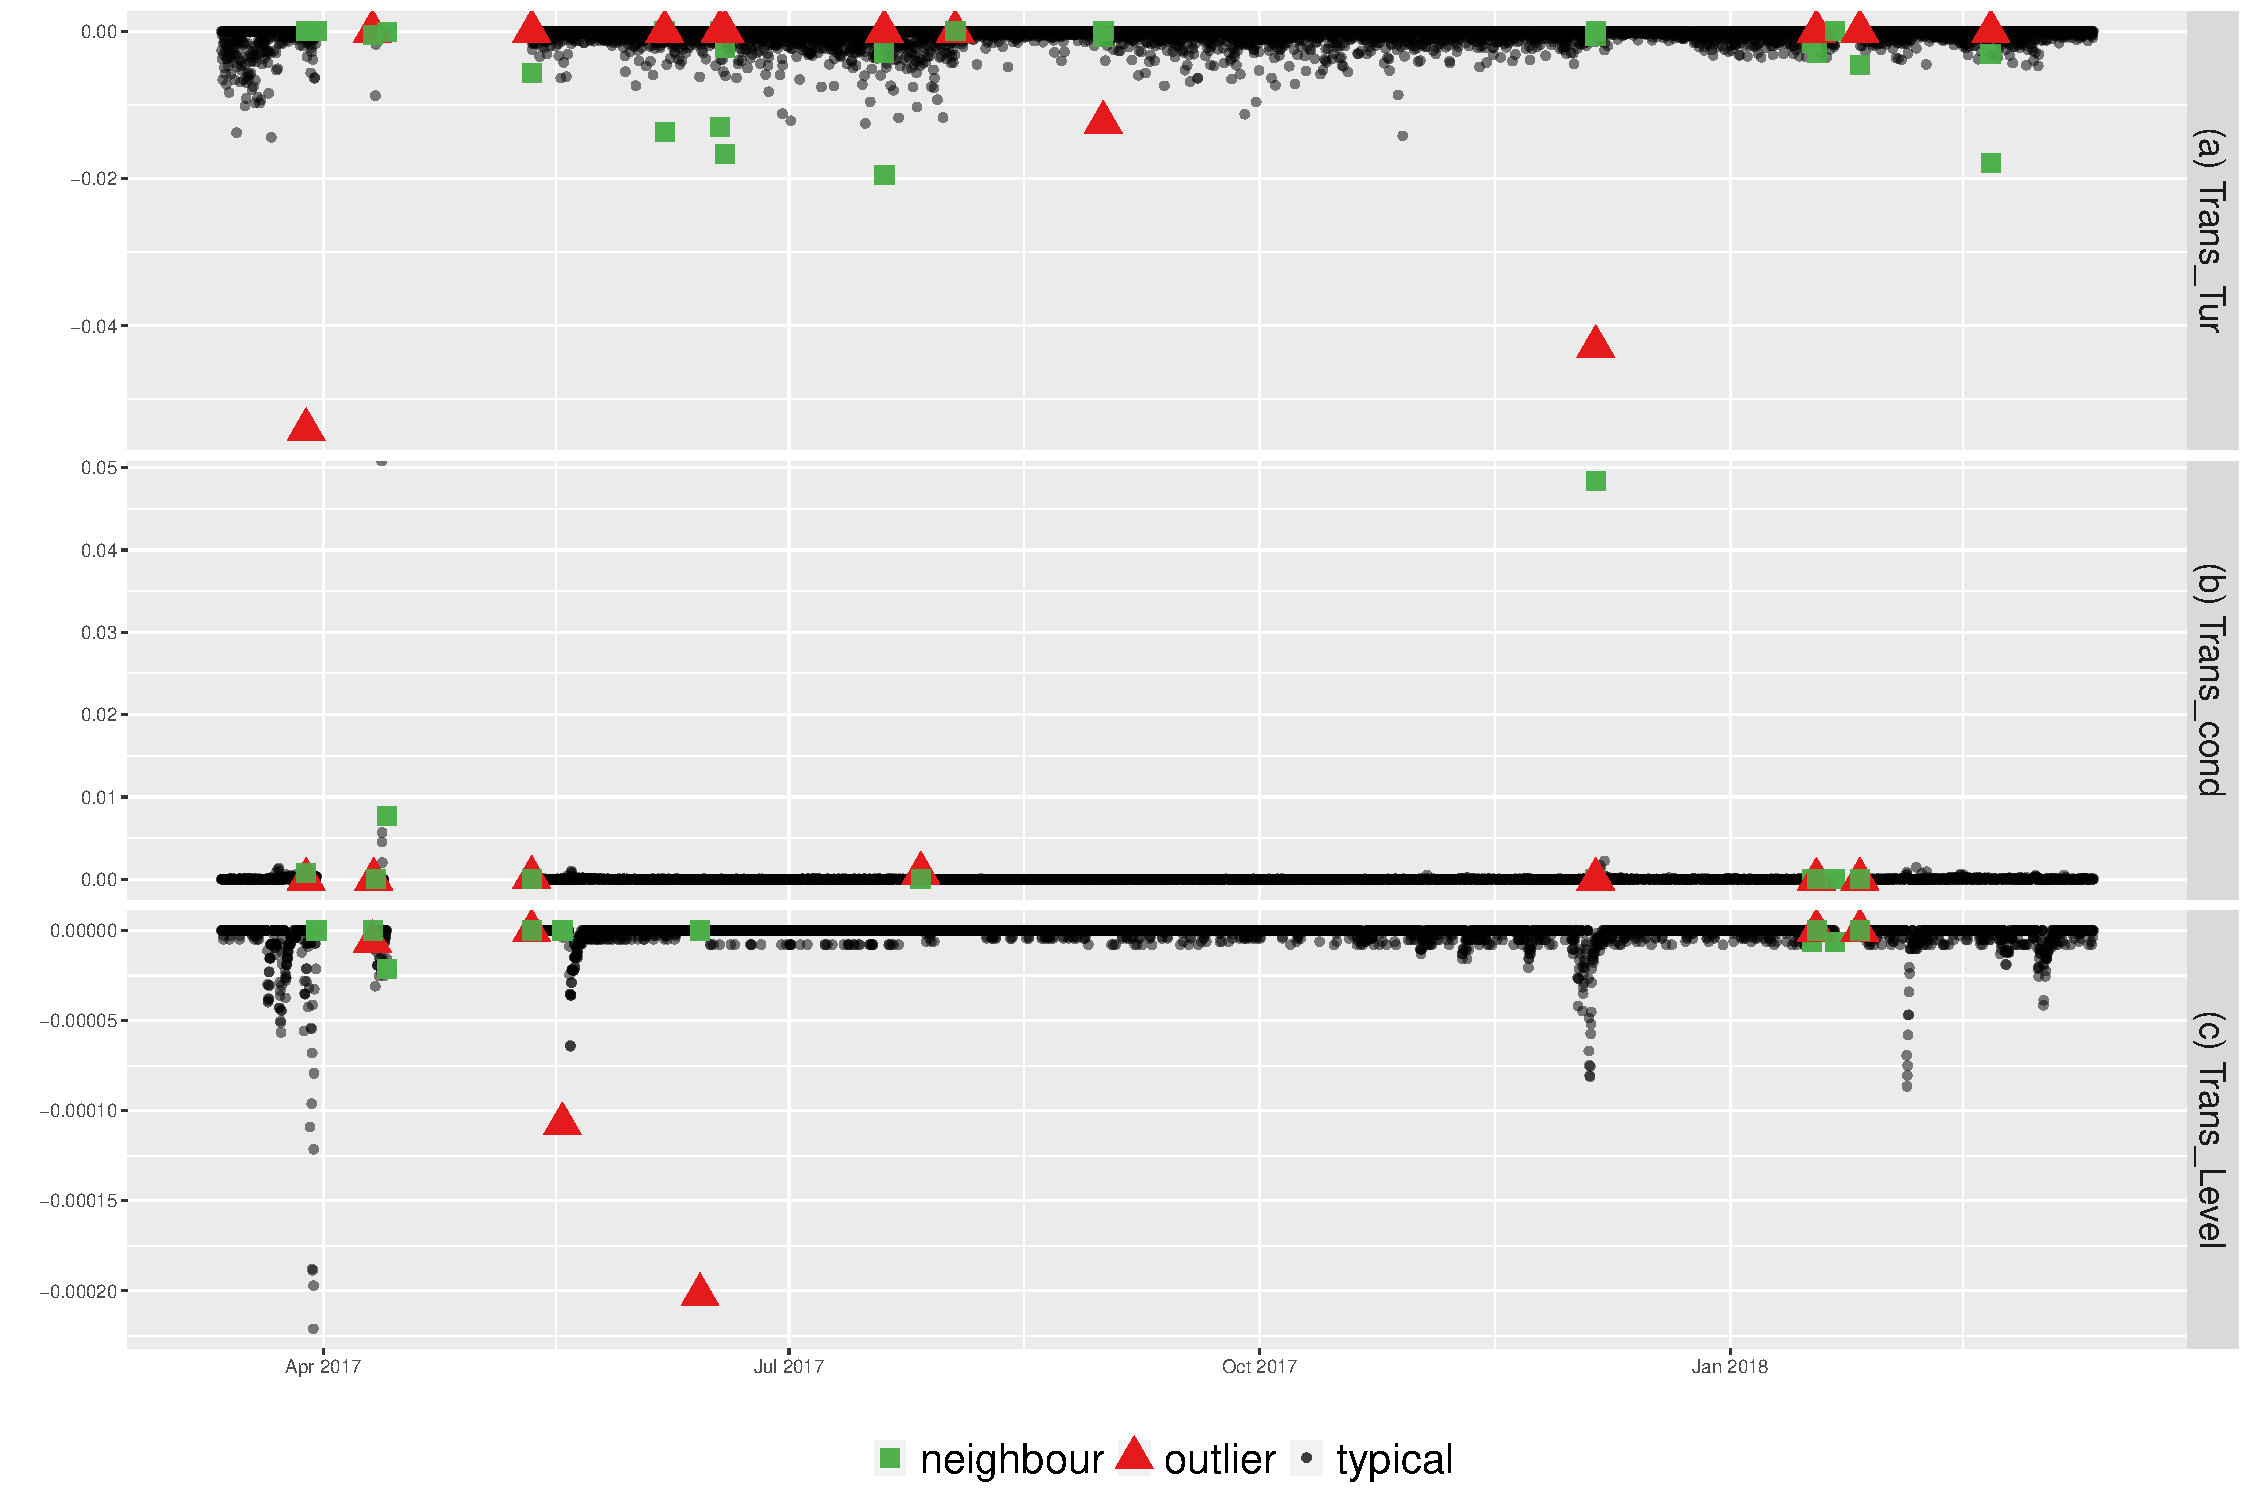
\includegraphics[width=1\textwidth]{./fig/transdemoTCLPioneertrans-1.pdf}

}

\caption{Transformed series (one sided derivatives) of turbidity (NTU), conductivity ($\mu$S/cm) and river level (m) measured by \textit{in situ} sensors at Pioneer River. In each plot, outliers determined by water-quality experts are shown in red, while typical points are shown in black. \color{black} Neighboring points are marked in green \color{black}}\label{fig:transdemoTCLpioneerPng}
\end{figure}

\begin{figure}[H]

{\centering 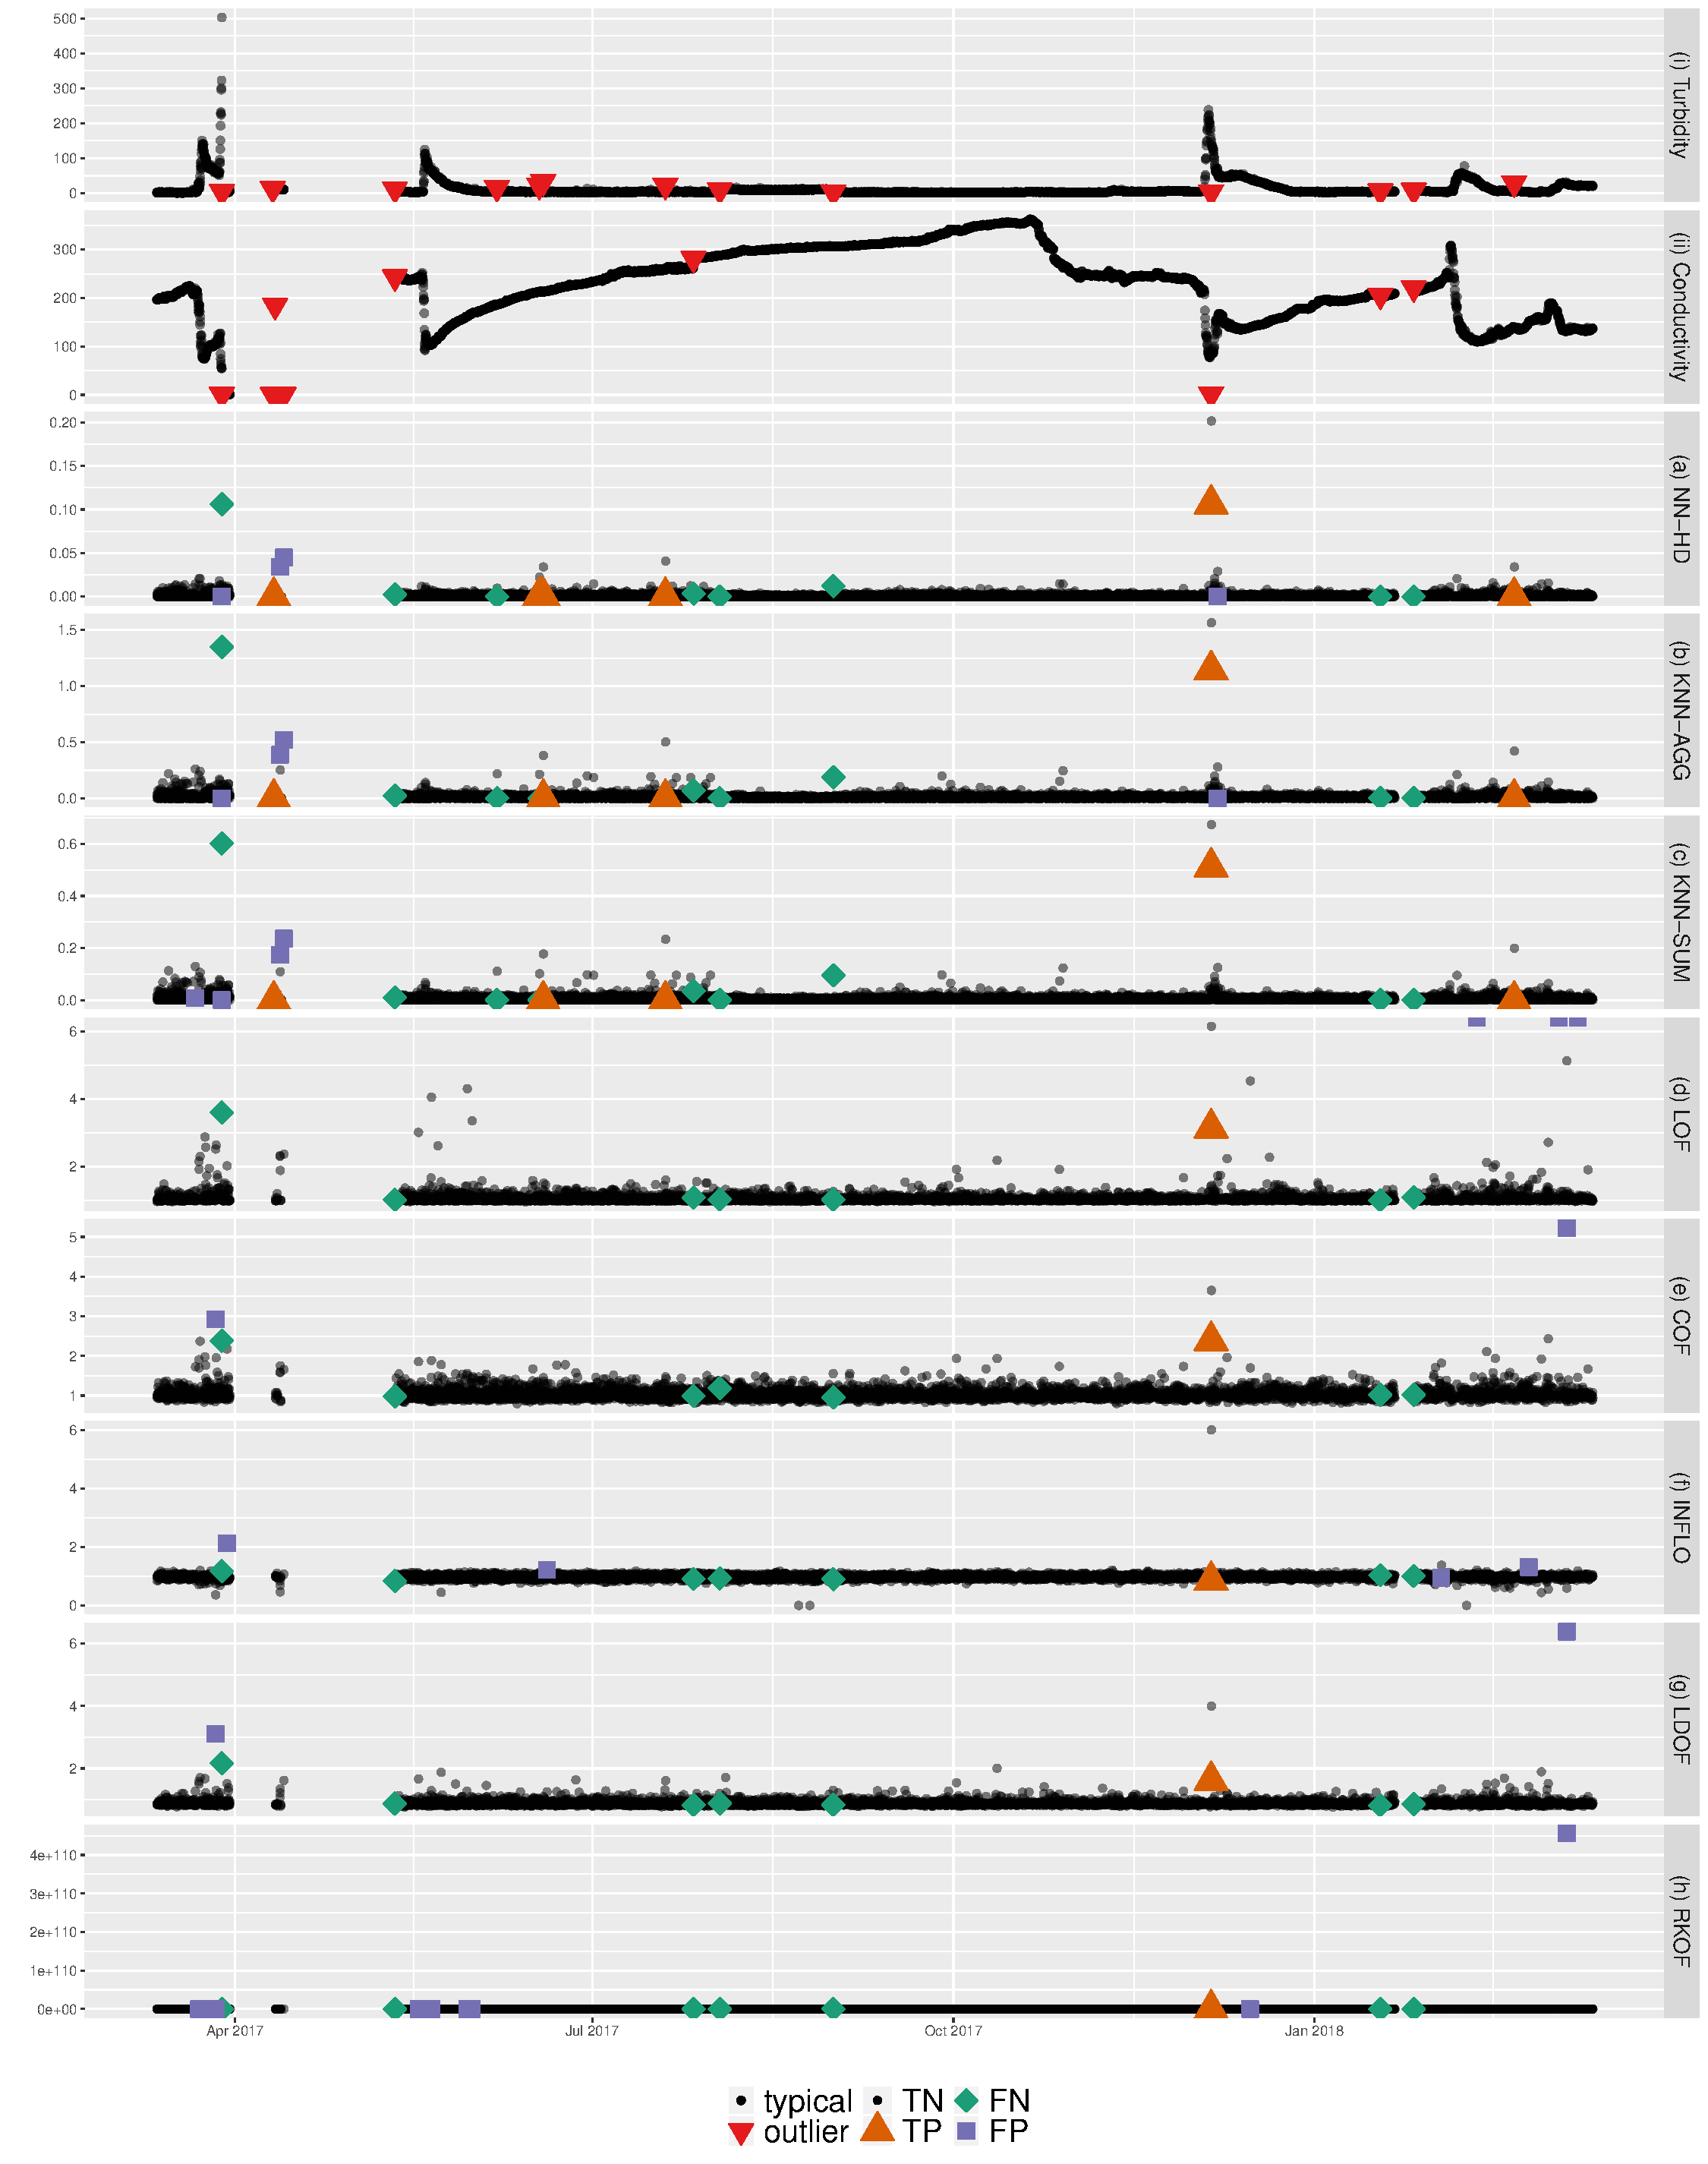
\includegraphics[width=1\linewidth,height=0.8\textheight]{./fig/onesidedderivativeTCpioneer-1.pdf}

}

\caption{Classification of outlier scores produced from different algorithms as true negatives (TN), true positives (TP), false negatives (FN), false positives (FP). The top two panels (i and ii) correspond to the original series (turbidity and conductivity) measured by \textit{in situ} sensors at Pioneer River. The target outliers (detected by water-quality experts) are shown in red, while typical points are shown in black. The remaining panels (a--h) give outlier scores produced by different outlier detection algorithms for high dimensional data when applied to the transformed series (one sided derivative) of the two variables: turbidity and conductivity. \color{black} Through different outlier scoring algorithms (Panel a - h) we are evaluating whether each point in time is an outlier or not. Therefore, from Panel a-h, if the outlier scoring algorithm is effective, then there should be either TP or TN  at each point in time when either a red triangle is plotted in at least one of the two panels (i- ii), or  black dots are plotted  in both of the top two panels (i - ii), respectively. Since outlier scores are non negative and are mostly clustered near zero, with some occasional high values, a square root transformation was applied to reduce skewness of the data in Panel (a) to (h). \color{black}}\label{fig:oneSidedDerivativeTCPioneerPng}
\end{figure}

\begin{table}[!htbp]

\caption{\label{tab:pioneerTable}Performance metrics of outlier
      detection algorithms performed on multivariate water-quality time series
      data (T, turbidity; C, conductivity; L, river level) from in situ sensors at Pioneer River, arranged in descending
      order of OP values. See Sections 2.7-8 for performance metric codes and details.}
\centering
\resizebox{\linewidth}{!}{
\begin{tabular}{rlllrrrrrrrrrrrr}
\toprule
i & Variables & Transformation & Method & TN & FN & FP & TP & Accuracy & GM & OP & PPV & NPV & min\_t & mu\_t & max\_t\\
\midrule
1 & T-C & One sided Derivative & \color{black} NN-HD \color{black} & 6226 & 10 & 5 & 39 & 0.9976 & 492.76 & 0.88 & 0.89 & 0.9984 & 128.0 & 136.5 & 257.7\\
2 & T-C & One sided Derivative & KNN-AGG & 6227 & 10 & 4 & 39 & 0.9978 & 492.80 & 0.88 & 0.91 & 0.9984 & 443.5 & 478.8 & 564.6\\
3 & T-C & One sided Derivative & KNN-SUM & 6227 & 10 & 4 & 39 & 0.9978 & 492.80 & 0.88 & 0.91 & 0.9984 & 209.6 & 222.2 & 325.5\\
4 & T-C & First Derivative & \color{black} NN-HD \color{black}  & 6229 & 12 & 2 & 37 & 0.9978 & 480.08 & 0.86 & 0.95 & 0.9981 & 169.6 & 182.0 & 272.3\\
5 & T-C & First Derivative & KNN-AGG & 6229 & 12 & 2 & 37 & 0.9978 & 480.08 & 0.86 & 0.95 & 0.9981 & 449.5 & 488.5 & 588.2\\
\addlinespace
6 & T-C & First Derivative & KNN-SUM & 6229 & 12 & 2 & 37 & 0.9978 & 480.08 & 0.86 & 0.95 & 0.9981 & 212.1 & 225.3 & 325.9\\
7 & T-C & First Derivative & INFLO & 6225 & 12 & 6 & 37 & 0.9971 & 479.92 & 0.86 & 0.86 & 0.9981 & 1452.1 & 1525.0 & 1613.2\\
8 & T-C & First Derivative & RKOF & 6224 & 12 & 7 & 37 & 0.9970 & 479.88 & 0.86 & 0.84 & 0.9981 & 400.2 & 430.4 & 523.9\\
9 & T-C-L & One sided Derivative & KNN-AGG & 6225 & 12 & 4 & 39 & 0.9975 & 492.72 & 0.86 & 0.91 & 0.9981 & 437.4 & 465.2 & 541.6\\
10 & T-C-L & One sided Derivative & KNN-SUM & 6225 & 12 & 4 & 39 & 0.9975 & 492.72 & 0.86 & 0.91 & 0.9981 & 195.6 & 214.5 & 297.8\\
\addlinespace
11 & T-C-L & First Derivative & RKOF & 6211 & 13 & 18 & 38 & 0.9951 & 485.82 & 0.85 & 0.68 & 0.9979 & 396.9 & 425.9 & 503.4\\
12 & T-C-L & First Derivative & KNN-AGG & 6227 & 14 & 2 & 37 & 0.9975 & 480.00 & 0.84 & 0.95 & 0.9978 & 460.8 & 478.0 & 570.3\\
13 & T-C-L & First Derivative & KNN-SUM & 6227 & 14 & 2 & 37 & 0.9975 & 480.00 & 0.84 & 0.95 & 0.9978 & 201.5 & 220.0 & 292.2\\
14 & T-C & First Derivative & COF & 6230 & 13 & 1 & 36 & 0.9978 & 473.58 & 0.84 & 0.97 & 0.9979 & 7812.7 & 7908.2 & 8453.3\\
15 & T-C & First Derivative & LDOF & 6230 & 13 & 1 & 36 & 0.9978 & 473.58 & 0.84 & 0.97 & 0.9979 & 23241.0 & 23435.7 & 24522.1\\
\addlinespace
16 & T-C & First Derivative & LOF & 6228 & 13 & 3 & 36 & 0.9975 & 473.51 & 0.84 & 0.92 & 0.9979 & 562.6 & 594.4 & 668.3\\
17 & T-C & One sided Derivative & INFLO & 6227 & 13 & 4 & 36 & 0.9973 & 473.47 & 0.84 & 0.90 & 0.9979 & 1488.8 & 1559.9 & 1633.1\\
18 & T-C & One sided Derivative & COF & 6229 & 13 & 2 & 36 & 0.9976 & 473.54 & 0.84 & 0.95 & 0.9979 & 7393.6 & 7505.5 & 8037.1\\
19 & T-C & One sided Derivative & LDOF & 6228 & 13 & 3 & 36 & 0.9975 & 473.51 & 0.84 & 0.92 & 0.9979 & 22802.2 & 22986.0 & 23561.3\\
20 & T-C & One sided Derivative & LOF & 6228 & 13 & 3 & 36 & 0.9975 & 473.51 & 0.84 & 0.92 & 0.9979 & 581.9 & 596.9 & 682.6\\
\addlinespace
21 & T-C & One sided Derivative & RKOF & 6219 & 13 & 12 & 36 & 0.9960 & 473.16 & 0.84 & 0.75 & 0.9979 & 388.6 & 419.7 & 510.4\\
22 & T-C & Original Series & INFLO & 6227 & 13 & 4 & 36 & 0.9973 & 473.47 & 0.84 & 0.90 & 0.9979 & 1405.6 & 1498.5 & 1578.2\\
23 & T-C-L & First Derivative & COF & 6228 & 15 & 1 & 36 & 0.9975 & 473.51 & 0.83 & 0.97 & 0.9976 & 7823.0 & 7910.7 & 8344.7\\
24 & T-C-L & First Derivative & LDOF & 6228 & 15 & 1 & 36 & 0.9975 & 473.51 & 0.83 & 0.97 & 0.9976 & 23220.1 & 23357.7 & 23878.3\\
25 & T-C-L & One sided Derivative & \color{black} NN-HD \color{black}  & 6228 & 15 & 1 & 36 & 0.9975 & 473.51 & 0.83 & 0.97 & 0.9976 & 125.7 & 131.9 & 206.1\\
\addlinespace
26 & T-C & Original Series & \color{black} NN-HD \color{black}  & 6230 & 14 & 1 & 35 & 0.9976 & 466.96 & 0.83 & 0.97 & 0.9978 & 159.9 & 171.0 & 278.2\\
27 & T-C & Original Series & KNN-AGG & 6226 & 14 & 5 & 35 & 0.9970 & 466.81 & 0.83 & 0.88 & 0.9978 & 434.2 & 468.7 & 553.0\\
28 & T-C & Original Series & KNN-SUM & 6226 & 14 & 5 & 35 & 0.9970 & 466.81 & 0.83 & 0.88 & 0.9978 & 192.9 & 211.6 & 305.8\\
29 & T-C & Original Series & COF & 6231 & 14 & 0 & 35 & 0.9978 & 467.00 & 0.83 & 1.00 & 0.9978 & 7518.5 & 7617.6 & 8501.1\\
30 & T-C & Original Series & LDOF & 6231 & 14 & 0 & 35 & 0.9978 & 467.00 & 0.83 & 1.00 & 0.9978 & 22770.9 & 22910.4 & 23857.1\\
\addlinespace
31 & T-C & Original Series & LOF & 6231 & 14 & 0 & 35 & 0.9978 & 467.00 & 0.83 & 1.00 & 0.9978 & 551.2 & 579.1 & 632.6\\
32 & T-C & Original Series & RKOF & 6222 & 14 & 9 & 35 & 0.9963 & 466.66 & 0.83 & 0.80 & 0.9978 & 373.6 & 401.9 & 475.4\\
33 & T-C-L & First Derivative & \color{black} NN-HD \color{black}  & 6227 & 15 & 2 & 36 & 0.9973 & 473.47 & 0.82 & 0.95 & 0.9976 & 157.3 & 167.1 & 244.3\\
34 & T-C-L & One sided Derivative & INFLO & 6226 & 15 & 3 & 36 & 0.9971 & 473.43 & 0.82 & 0.92 & 0.9976 & 1383.5 & 1418.8 & 1477.4\\
35 & T-C-L & One sided Derivative & COF & 6227 & 15 & 2 & 36 & 0.9973 & 473.47 & 0.82 & 0.95 & 0.9976 & 7414.6 & 7497.9 & 7899.6\\
\addlinespace
36 & T-C-L & One sided Derivative & LDOF & 6227 & 15 & 2 & 36 & 0.9973 & 473.47 & 0.82 & 0.95 & 0.9976 & 22756.8 & 23090.7 & 23941.1\\
37 & T-C-L & One sided Derivative & RKOF & 6214 & 15 & 15 & 36 & 0.9952 & 472.97 & 0.82 & 0.71 & 0.9976 & 390.5 & 422.1 & 490.3\\
38 & T-C-L & First Derivative & INFLO & 6229 & 16 & 0 & 35 & 0.9975 & 466.92 & 0.81 & 1.00 & 0.9974 & 1344.7 & 1398.3 & 1456.9\\
39 & T-C-L & First Derivative & LOF & 6229 & 16 & 0 & 35 & 0.9975 & 466.92 & 0.81 & 1.00 & 0.9974 & 585.6 & 600.7 & 688.1\\
40 & T-C-L & One sided Derivative & LOF & 6223 & 16 & 6 & 35 & 0.9965 & 466.70 & 0.81 & 0.85 & 0.9974 & 583.4 & 596.1 & 672.1\\
\addlinespace
41 & T-C-L & Original Series & \color{black} NN-HD \color{black}  & 6228 & 16 & 1 & 35 & 0.9973 & 466.88 & 0.81 & 0.97 & 0.9974 & 152.8 & 163.0 & 231.2\\
42 & T-C-L & Original Series & KNN-AGG & 6224 & 16 & 5 & 35 & 0.9967 & 466.73 & 0.81 & 0.88 & 0.9974 & 439.3 & 456.3 & 534.2\\
43 & T-C-L & Original Series & KNN-SUM & 6224 & 16 & 5 & 35 & 0.9967 & 466.73 & 0.81 & 0.88 & 0.9974 & 186.5 & 201.4 & 269.6\\
44 & T-C-L & Original Series & INFLO & 6229 & 16 & 0 & 35 & 0.9975 & 466.92 & 0.81 & 1.00 & 0.9974 & 1329.9 & 1372.8 & 1415.0\\
45 & T-C-L & Original Series & COF & 6229 & 16 & 0 & 35 & 0.9975 & 466.92 & 0.81 & 1.00 & 0.9974 & 7596.5 & 7707.2 & 8357.8\\
\addlinespace
46 & T-C-L & Original Series & LDOF & 6229 & 16 & 0 & 35 & 0.9975 & 466.92 & 0.81 & 1.00 & 0.9974 & 22897.7 & 127337.1 & 10458496.0\\
47 & T-C-L & Original Series & LOF & 6229 & 16 & 0 & 35 & 0.9975 & 466.92 & 0.81 & 1.00 & 0.9974 & 549.5 & 580.9 & 646.9\\
48 & T-C-L & Original Series & RKOF & 6217 & 16 & 12 & 35 & 0.9955 & 466.47 & 0.81 & 0.74 & 0.9974 & 368.3 & 406.8 & 497.2\\
\bottomrule
\end{tabular}}
\end{table}

\section{Discussion}\label{sec:discussion}

We introduced a new \color{black} procedure, named oddwater procedure \color{black} for the detection of outliers in
water-quality data from \emph{in~situ} sensors, where outliers were
specifically defined as due to technical errors that make the data
unreliable and untrustworthy. We showed that our \color{black} oddwater procedure, \color{black}
with carefully selected data transformation methods derived from data
features, can greatly assist in increasing the performance of a range of
existing outlier detection algorithms. Our \color{black} oddwater procedure, \color{black} and analysis using
data obtained from \emph{in~situ} sensors positioned at two study sites,
Sandy Creek and Pioneer River, performed well with outlier types such as
sudden isolated spikes, sudden isolated drops, and level shifts, while
maintaining low false detection rates. As an unsupervised \color{black} procedure, \color{black} our
approach can be easily extended to other water-quality variables, other
sites and also to other outlier detection tasks in other application
domains. The only requirement is to select suitable transformation
methods according to the data features that differentiate the outlying
instances from the typical behaviors of a given system.

Studies have shown that transforming variables affects densities,
relative distances and orientation of points within the data space and
therefore can improve the ability to perceive patterns in the data which
are not clearly visible in the original data space
\citep{dang2014transforming}. This was the case in our study, where
no clear separation was visible between outliers and typical data points
in the original data space, but a clear separation was obtained between
the two sets of points once the one-sided derivative transformation was
applied to the original series. Having this type of a separation between
outliers and typical points is important before applying unsupervised
outlier detection algorithms for high dimensional data because the methods
are usually based on the definition of outliers in terms of distance or
density \citep{talagala2018anomaly}. Most of the outlier detection
algorithms (KNN-SUM, KNN-AGG, \color{black} NN-HD \color{black}, COF, LOF and INFLO) performed
least well with the untransformed original series, demonstrating how
data transformation methods can assist in improving the ability of
outlier detection algorithms while maintaining low false detection
rates.

Although outlying points were clearly separated from their majority,
which corresponded to the typical behaviors, the individual outliers
were not isolated and were surrounded by the other outlying points.
Because \color{black} NN-HD \color{black} has the additional requirement of isolation in
addition to clear separation between outlying points and typical points,
it performed poorly in comparison to the two KNN distance-based
algorithms (KNN-AGG and KNN-SUM) which are not restricted to the single
most nearest neighbor \citep{talagala2018anomaly}. For the current
work \(k\) was set to 10, the maximum default value of \(k\) in
\citet{madsen2018ddoutlier}, because too large a value of \(k\) could
skew the focus towards global outliers (points that deviates significantly from the rest of the dataset) alone \citep{zhang2009new} and
make the algorithms computationally inefficient. On the other hand, too
small a value of \(k\) could incorporate an additional assumption of
isolation into the algorithm, as in the \color{black} NN-HD algorithm \color{black} where \(k=1\).
Among the analysis using transformed series, LOF with the first
derivative transformation performed the least well, which could also be due
to its additional assumption of isolation \citep{tang2002enhancing}. \color{black} However, using the same \(k\)  across all algorithms may bias direct comparison as the performance of the algorithms can depend on the value of  \(k\) and algorithms can reach their peak performance for different choices of  \(k\)  \citep{campos2016evaluation}. Therefore performing an optimisation to select the best \(k\)  is non trivial and we leave it for future work. \color{black}

We took the correlation structure between the variables into account when detecting outliers as some were apparent only in the high dimensional space but not when each variable was considered independently
\citep{ben2005outlier}. A negative relationship was observed between
conductivity and turbidity and also between conductivity and level for
the Sandy Creek data. However, for Pioneer River, no clear relationship
was observed between level and the remaining two variables, turbidity
and conductivity. This could be one reason why the variable combination
with river level gave poor results for the Pioneer River dataset, while
results for other combinations were similar to those of Sandy Creek.

The one-sided derivative transformation outperformed the derivative
transformation. This was expected because in an occurrence of a sudden
spike or isolated drop the first derivative assigns high values to two
consecutive points, the actual outlying point as well as the neighboring
point, and therefore increases the false positive rate (because the
neighboring points that are declared to be outliers actually correspond
to typical points in the original data space).

Our goal was to detect
suitable transformations, combinations of variables, and the algorithms
for outlier score calculation for the data from two study sites. Results may depend on the characteristics of the time series (site and time
dependent for example), and what is best for one site may not be the
best for another site. Therefore care should be taken to select
transformations most suitable for the problem at hand. According to
\citet{dang2014transforming}, any transformation used on a dataset
must be evaluated in terms of a figure of merit \color{black} (i.e. a numerical quantity used to characterize the performance of a method, relative to its alternatives). \color{black}  For our work on
detecting outliers, the figure of merit was the maximum separability of
the two classes generated by outliers and typical points. However, we
acknowledge that the set of transformations that we used for this work
was relatively limited and influenced by the data obtained from the two
study sites. Therefore, the set of transformations we considered (Table
\ref{table:table_1}) should be viewed only as an illustration of our
\color{black} oddwater procedure \color{black} for detecting outliers. We expect that the set of
transformations will expand over time as the \color{black} oddwater procedure \color{black} is used for other
data from other study sites and for applications to other fields.

\color{black}
For the current work we selected
transformation methods that could highlight  abrupt changes in the
water-quality data.We hope to expand the ability of oddwater procedure  so that it can
detect other outlier types not previously targeted but commonly observed
in water quality data \color{black} (e.g.: low/high variability, drift etc. as per \citet{leigh2019framework}). One possibility is to consider the residuals
at each point, defined as the difference between the actual values and
the fitted values (similar to \citet{schwarz2008wind}) or the
difference between the actual values and the predicted values (similar
to \citet{hill2006automated}), as a transformation and apply outlier
detection algorithms to the high dimensional space defined by the residuals.
Here the challenge will be to identify the appropriate curve fitting and
prediction models to generate the residual series. In this way,
continuous subsequences of high values could correspond to other kinds of technical outliers such as high variability or drift. However, the range of applications and the space of the transformations are extremely diverse, which makes it challenging to provide a structured
formal vision that covers all of the possible transformations that could be considered. The transformations we presented in this paper were mainly  chosen  as appropriate to the data collected from Sandy Creek and Pioneer River.
We observed that different transformations can lead to entirely different data structures and that the selection of suitable transformations is directed by the data features and typical patterns imposed by a given application. Domain specific knowledge plays a vital role when selecting suitable transformations and as such defining structured guidelines
for the selection of suitable transformations remains problematic.
\color{black}

Not surprisingly, \color{black} NN-HD \color{black} algorithm required the least computational
time given the outlying score calculation only involves searching for
the single most nearest neighbors of each test point
\citep{wilkinsonvisualizing}. The mean computational time of KNN-AGG
was twice as high as that of KNN-SUM because the KNN-AGG algorithm has
the additional requirement of calculating weights that assign nearest
neighbors higher weight relative to the neighbors farther apart
\citep{angiulli2002fast}. LOF and its extensions (INFLO, COF and
LDOF) required the most computational time; all four algorithms involve
a two step searching mechanism at each test point when calculating the
corresponding outlying score. This means that at each test point each
algorithm searches its \(k\) nearest neighbors as well those of the
detected nearest neighbors for the outlier score calculation
\citep{breunig2000lof,tang2002enhancing,jin2006ranking,zhang2009new}.

We hope to extend our multivariate outlier detection framework into space and time
so that it can deal with the spatio-temporal correlation structure along
branching river networks. \color{black} Further, in the current paper we have introduced our oddwater procedure as a batch method. However, due to the unsupervised nature of our oddwater procedure it can be easily extended to a streaming data scenario with the help of a sliding window of fixed length. A streaming data scenario always demands a near-real-time support. Therefore one significant challenge is to find efficient  methods  that allow us to update  outlier scores taking account of the newest observations and removing the oldest observations introduced by overlapping sliding windows, rather than recalculating scores corresponding to observations which are not affected by either  new arrivals or the oldest observations (that are  no longer covered by the latest window). Further work will be needed to investigate the  efficient computation of regenerating nearest neighbours in a data streaming context. \color{black}

%Text here ===>>>

%%

%  Numbered lines in equations:
%  To add line numbers to lines in equations,
%  \begin{linenomath*}
%  \begin{equation}
%  \end{equation}
%  \end{linenomath*}

%% Enter Figures and Tables near as possible to where they are first mentioned:
%
% DO NOT USE \psfrag or \subfigure commands.
%
% Figure captions go below the figure.
% Table titles go above tables;  other caption information
%  should be placed in last line of the table, using
% \multicolumn2l{$^a$ This is a table note.}
%
%----------------
% EXAMPLE FIGURE
%
% \begin{figure}[h]
% \centering
% when using pdflatex, use pdf file:
% \includegraphics[width=20pc]{figsamp.pdf}
%
% when using dvips, use .eps file:
% \includegraphics[width=20pc]{figsamp.eps}
%
% \caption{Short caption}
% \label{figone}
%  \end{figure}
%
% ---------------
% EXAMPLE TABLE
%
% \begin{table}
% \caption{Time of the Transition Between Phase 1 and Phase 2$^{a}$}
% \centering
% \begin{tabular}{l c}
% \hline
%  Run  & Time (min)  \\
% \hline
%   $l1$  & 260   \\
%   $l2$  & 300   \\
%   $l3$  & 340   \\
%   $h1$  & 270   \\
%   $h2$  & 250   \\
%   $h3$  & 380   \\
%   $r1$  & 370   \\
%   $r2$  & 390   \\
% \hline
% \multicolumn{2}{l}{$^{a}$Footnote text here.}
% \end{tabular}
% \end{table}

%% SIDEWAYS FIGURE and TABLE
% AGU prefers the use of {sidewaystable} over {landscapetable} as it causes fewer problems.
%
% \begin{sidewaysfigure}
% \includegraphics[width=20pc]{figsamp}
% \caption{caption here}
% \label{newfig}
% \end{sidewaysfigure}
%
%  \begin{sidewaystable}
%  \caption{Caption here}
% \label{tab:signif_gap_clos}
%  \begin{tabular}{ccc}
% one&two&three\\
% four&five&six
%  \end{tabular}
%  \end{sidewaystable}

%% If using numbered lines, please surround equations with \begin{linenomath*}...\end{linenomath*}
%\begin{linenomath*}
%\begin{equation}
%y|{f} \sim g(m, \sigma),
%\end{equation}
%\end{linenomath*}

%%% End of body of article

%%%%%%%%%%%%%%%%%%%%%%%%%%%%%%%%
%% Optional Appendix goes here
%
% The \appendix command resets counters and redefines section heads
%
% After typing \appendix
%
%\section{Here Is Appendix Title}
% will show
% A: Here Is Appendix Title
%

%\section{Here is a sample appendix}

%%%%%%%%%%%%%%%%%%%%%%%%%%%%%%%%%%%%%%%%%%%%%%%%%%%%%%%%%%%%%%%%
%
% Optional Glossary, Notation or Acronym section goes here:
%
%%%%%%%%%%%%%%
% Glossary is only allowed in Reviews of Geophysics
%  \begin{glossary}
%  \term{Term}
%   Term Definition here
%  \term{Term}
%   Term Definition here
%  \term{Term}
%   Term Definition here
%  \end{glossary}

%
%%%%%%%%%%%%%%
% Acronyms
%   \begin{acronyms}
%   \acro{Acronym}
%   Definition here
%   \acro{EMOS}
%   Ensemble model output statistics
%   \acro{ECMWF}
%   Centre for Medium-Range Weather Forecasts
%   \end{acronyms}

%
%%%%%%%%%%%%%%
% Notation
%   \begin{notation}
%   \notation{$a+b$} Notation Definition here
%   \notation{$e=mc^2$}
%   Equation in German-born physicist Albert Einstein's theory of special
%  relativity that showed that the increased relativistic mass ($m$) of a
%  body comes from the energy of motion of the body—that is, its kinetic
%  energy ($E$)—divided by the speed of light squared ($c^2$).
%   \end{notation}

%%%%%%%%%%%%%%%%%%%%%%%%%%%%%%%%%%%%%%%%%%%%%%%%%%%%%%%%%%%%%%%%
%
%  ACKNOWLEDGMENTS
%
% The acknowledgments must list:
%
% >>>>	A statement that indicates to the reader where the data
% 	supporting the conclusions can be obtained (for example, in the
% 	references, tables, supporting information, and other databases).
%
% 	All funding sources related to this work from all authors
%
% 	Any real or perceived financial conflicts of interests for any
%	author
%
% 	Other affiliations for any author that may be perceived as
% 	having a conflict of interest with respect to the results of this
% 	paper.
%
%
% It is also the appropriate place to thank colleagues and other contributors.
% AGU does not normally allow dedications.

\acknowledgments

Funding for this project was provided by the Queensland Department of
Environment and Science (DES) and the ARC Centre of Excellence for
Mathematical and Statistical Frontiers (ACEMS). The authors would like
to acknowledge the Queensland Department of Environment and Science; in
particular, the Great Barrier Reef Catchment Loads Monitoring Program
for the data, and the staff from Water Quality and Investigations for
their input. We thank Ryan S. Turner and Erin E. Peterson for several
valuable discussions regarding project requirements and water quality
characteristics. Further, this research was supported in part by the Monash eResearch Centre and eSolutions-Research Support Services through the use of the MonARCH (Monash Advanced Research Computing Hybrid) HPC Cluster. We would also like to thank David Hill and other anonymous reviewers
for  their valuable comments and suggestions. The datasets used for this article are available in the
open source R package \texttt{oddwater} \citep{oddwater2018}.

%% ------------------------------------------------------------------------ %%
%% References and Citations

%%%%%%%%%%%%%%%%%%%%%%%%%%%%%%%%%%%%%%%%%%%%%%%
% BibTeX is preferred:
%
\bibliography{bibliography.bib}
%
% no need to specify bibliographystyle
%%%%%%%%%%%%%%%%%%%%%%%%%%%%%%%%%%%%%%%%%%%%%%%

%\appendix
%\section*{Appendix}

% Please use ONLY \citet and \citep for reference citations.
% DO NOT use other cite commands (e.g., \cite, \citeyear, \nocite, \citealp, etc.).
%% Example \citet and \citep:
%  ...as shown by \citet{Boug10}, \citet{Buiz07}, \citet{Fra10},
%  \citet{Ghel00}, and \citet{Leit74}.

%  ...as shown by \citep{Boug10}, \citep{Buiz07}, \citep{Fra10},
%  \citep{Ghel00, Leit74}.

%  ...has been shown \citep [e.g.,][]{Boug10,Buiz07,Fra10}.

\end{document}

More Information and Advice:

%% ------------------------------------------------------------------------ %%
%
%  SECTION HEADS
%
%% ------------------------------------------------------------------------ %%

% Capitalize the first letter of each word (except for
% prepositions, conjunctions, and articles that are
% three or fewer letters).

% AGU follows standard outline style; therefore, there cannot be a section 1 without
% a section 2, or a section 2.3.1 without a section 2.3.2.
% Please make sure your section numbers are balanced.
% ---------------
% Level 1 head
%
% Use the \section{} command to identify level 1 heads;
% type the appropriate head wording between the curly
% brackets, as shown below.
%
%An example:
%\section{Level 1 Head: Introduction}
%
% ---------------
% Level 2 head
%
% Use the \subsection{} command to identify level 2 heads.
%An example:
%\subsection{Level 2 Head}
%
% ---------------
% Level 3 head
%
% Use the \subsubsection{} command to identify level 3 heads
%An example:
%\subsubsection{Level 3 Head}
%
%---------------
% Level 4 head
%
% Use the \subsubsubsection{} command to identify level 3 heads
% An example:
%\subsubsubsection{Level 4 Head} An example.
%
%% ------------------------------------------------------------------------ %%
%
%  IN-TEXT LISTS
%
%% ------------------------------------------------------------------------ %%
%
% Do not use bulleted lists; enumerated lists are okay.
% \begin{enumerate}
% \item
% \item
% \item
% \end{enumerate}
%
%% ------------------------------------------------------------------------ %%
%
%  EQUATIONS
%
%% ------------------------------------------------------------------------ %%

% Single-line equations are centered.
% Equation arrays will appear left-aligned.

Math coded inside display math mode \[ ...\]
 will not be numbered, e.g.,:
 \[ x^2=y^2 + z^2\]

 Math coded inside \begin{equation} and \end{equation} will
 be automatically numbered, e.g.,:
 \begin{equation}
 x^2=y^2 + z^2
 \end{equation}

% To create multiline equations, use the
% \begin{eqnarray} and \end{eqnarray} environment
% as demonstrated below.
\begin{eqnarray}
  x_{1} & = & (x - x_{0}) \cos \Theta \nonumber \\
        && + (y - y_{0}) \sin \Theta  \nonumber \\
  y_{1} & = & -(x - x_{0}) \sin \Theta \nonumber \\
        && + (y - y_{0}) \cos \Theta.
\end{eqnarray}

%If you don't want an equation number, use the star form:
%\begin{eqnarray*}...\end{eqnarray*}
Click to hide the PDF

% Break each line at a sign of operation
% (+, -, etc.) if possible, with the sign of operation
% on the new line.

% Indent second and subsequent lines to align with
% the first character following the equal sign on the
% first line.

% Use an \hspace{} command to insert horizontal space
% into your equation if necessary. Place an appropriate
% unit of measure between the curly braces, e.g.
% \hspace{1in}; you may have to experiment to achieve
% the correct amount of space.

%% ------------------------------------------------------------------------ %%
%
%  EQUATION NUMBERING: COUNTER
%
%% ------------------------------------------------------------------------ %%

% You may change equation numbering by resetting
% the equation counter or by explicitly numbering
% an equation.

% To explicitly number an equation, type \eqnum{}
% (with the desired number between the brackets)
% after the \begin{equation} or \begin{eqnarray}
% command. The \eqnum{} command will affect only
% the equation it appears with; LaTeX will number
% any equations appearing later in the manuscript
% according to the equation counter.
%

% If you have a multiline equation that needs only
% one equation number, use a \nonumber command in
% front of the double backslashes (\\) as shown in
% the multiline equation above.

% If you are using line numbers, remember to surround
% equations with \begin{linenomath*}...\end{linenomath*}

%  To add line numbers to lines in equations:
%  \begin{linenomath*}
%  \begin{equation}
%  \end{equation}
%  \end{linenomath*}

